\documentclass[a4paper, 16pt]{article}
\usepackage{geometry}
\usepackage{tikz}
\usepackage{tcolorbox}
\usepackage[utf8]{inputenc}  % required
\usepackage[T1]{fontenc}
\usepackage{amsmath}
\usepackage{lmodern}

\geometry{margin=1.5cm}
\newcommand{\chbox}[1]{
\begin{tcolorbox}[
 colback=green!10,
 colframe=green!50!black,
 boxrule=0.5pt,
 arc=4pt
]
#1
\end{tcolorbox}
}

\newcommand{\infbox}[1]{
\begin{tcolorbox}[
 colback=cyan!10,
 colframe=cyan!50!black,
 boxrule=0.5pt,
 arc=4pt
]
#1
\end{tcolorbox}
}


\newcommand{\tbox}[1]{
\begin{tcolorbox}[
 colback=gray!0,
 colframe=gray!50!black,
 boxrule=0.5pt,
 arc=4pt
]
\begin{center}
#1
\end{center}
\end{tcolorbox}
}


\newcommand{\circliste}[1]{
  \begin{tikzpicture}[every node/.style={draw, circle, minimum size=1cm, font=\small, inner sep=2pt}]
    
    % Calcul longueur
    \foreach \word [count=\n] in {#1} {
      \global\let\total\n
    }
    
    % Calcul rayon
    \pgfmathsetmacro{\radius}{6}
    
    % Placement noeuds
    \foreach \word [count=\i] in {#1} {
      \pgfmathsetmacro{\angle}{90 - (\i-1)*360/\total}
      \ifnum\i=1
        \node[draw=red, thick] (\i) at (\angle:\radius cm) {\word};
      \else
        \node (\i) at (\angle:\radius cm) {\word};
      \fi
    }
    
    % Dessin fleches
    \pgfmathtruncatemacro{\lastnode}{\total}
    \foreach \i in {1,...,\lastnode} {
      \pgfmathtruncatemacro{\next}{mod(\i,\total)+1}
      \draw[<->, shorten >=2pt, shorten <=2pt] (\i) to[bend right=25] (\next);
    }
  \end{tikzpicture}
}


\newcommand{\linliste}[1]{
  \begin{tikzpicture}[every node/.style={draw, circle, minimum size=1cm, font=\small, inner sep=2pt}]

    % max par ligne
    \pgfmathsetmacro{\rowsize}{6}
    
    % Calcul longueur
      \foreach \word [count=\n] in {#1} {
        \global\let\total\n
      }
      
      % Placement noeuds
      \foreach \word [count=\i] in {#1} {
        \pgfmathsetmacro{\quot}{-floor((\i-1)/\rowsize)}
        \pgfmathsetmacro{\xpos}{.9 * (1+pow(-1, \quot+1))*\rowsize + pow(-1, \quot) * mod(\i-1, \rowsize)*2}
        \pgfmathsetmacro{\ypos}{\quot*2}
        \node[scale=1] (\i) at (\xpos, \ypos) {\word};
      }
      
      % Dessin fleches
      \pgfmathtruncatemacro{\lastnode}{\total}
      \foreach \i in {1,...,\lastnode} {
        \pgfmathtruncatemacro{\next}{mod(\i,\total)+1}
        \ifnum\i<\lastnode
        \draw[<->, shorten >=2pt, shorten <=2pt] (\i) to (\next);
        \fi
      }
  \end{tikzpicture}
}

\begin{document}

\noindent\rule{\textwidth}{0.4pt}
\vspace{.3cm}
\noindent \textbf{Badr Benchekroun, Jade Ziani} \hfill \textbf{Université Gustave Eiffel} \\
\textbf{Initiation à la Prog C} \hfill \textbf{L2, 3ème semestre} \\
\begin{center}
\textbf{\Large Visualisation de l'ALDI} \\ 
\vspace{.2cm}
\textit{\large Algorithme d'insertion triée dans des listes circulaires}
\end{center}
\vspace{.2cm}
\noindent\rule{\textwidth}{0.4pt}

\vspace{.5cm}

Between the 15th and 13th centuries BC, the Hittites were one of the dominant powers of the Near East, coming into conflict with the New Kingdom of Egypt, the Middle Assyrian Empire, and the Empire of Mitanni. 
\section{« between »}
\begin{tcolorbox}[arc=5pt, colback=white!0, colframe=orange!50!black]
\infbox{
Insertion de \textbf{« between »}
}
\begin{center}
\tbox{
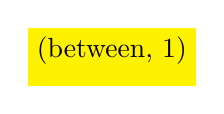
\begin{tikzpicture}
[
    level 1/.style={sibling distance=75mm, scale=1},
    level/.style={sibling distance=35mm, scale=.95},
]
\node [fill=yellow, scale=1.00]
{($\underset{\text{}}{\text{between}}$, 1)} 
;
\end{tikzpicture}
}
\end{center}

\end{tcolorbox}\section{« the »}
\begin{tcolorbox}[arc=5pt, colback=white!0, colframe=orange!50!black]
\infbox{
Insertion de \textbf{« the »}
}
\begin{center}
\tbox{
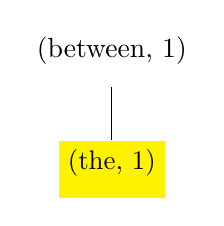
\begin{tikzpicture}
[
    level 1/.style={sibling distance=75mm, scale=1},
    level/.style={sibling distance=35mm, scale=.95},
]
\node [, scale=1.00]
{($\underset{\text{}}{\text{between}}$, 1)} 
    child {node[fill=yellow, scale=0.97]
{($\underset{\text{}}{\text{the}}$, 1)} 
};
\end{tikzpicture}
}
\end{center}

\end{tcolorbox}\section{« and »}
\begin{tcolorbox}[arc=5pt, colback=white!0, colframe=orange!50!black]
\infbox{
Insertion de \textbf{« and »}
}
\begin{center}
\tbox{
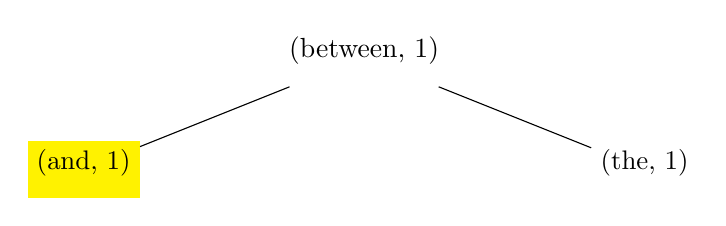
\begin{tikzpicture}
[
    level 1/.style={sibling distance=75mm, scale=1},
    level/.style={sibling distance=35mm, scale=.95},
]
\node [, scale=1.00]
{($\underset{\text{}}{\text{between}}$, 1)} 
    child {node[fill=yellow, scale=0.97]
{($\underset{\text{}}{\text{and}}$, 1)} 
}    child {node[, scale=0.97]
{($\underset{\text{}}{\text{the}}$, 1)} 
};
\end{tikzpicture}
}
\end{center}

\end{tcolorbox}\section{« centuries »}
\begin{tcolorbox}[arc=5pt, colback=white!0, colframe=orange!50!black]
\infbox{
Insertion de \textbf{« centuries »}
}
\begin{center}
\tbox{
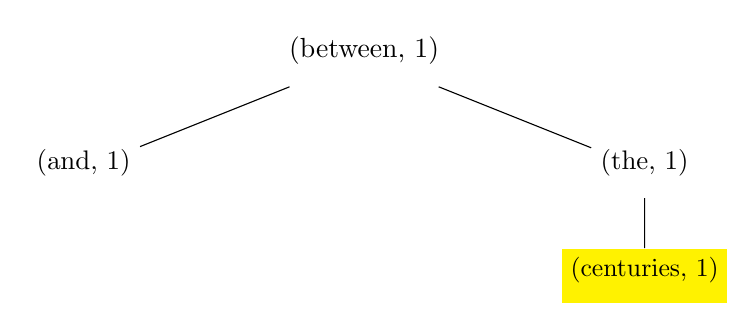
\begin{tikzpicture}
[
    level 1/.style={sibling distance=75mm, scale=1},
    level/.style={sibling distance=35mm, scale=.95},
]
\node [, scale=1.00]
{($\underset{\text{}}{\text{between}}$, 1)} 
    child {node[, scale=0.97]
{($\underset{\text{}}{\text{and}}$, 1)} 
}    child {node[, scale=0.97]
{($\underset{\text{}}{\text{the}}$, 1)} 
    child {node[fill=yellow, scale=0.93]
{($\underset{\text{}}{\text{centuries}}$, 1)} 
}};
\end{tikzpicture}
}
\end{center}

\end{tcolorbox}\section{« bc »}
\begin{tcolorbox}[arc=5pt, colback=white!0, colframe=orange!50!black]
\infbox{
Insertion de \textbf{« bc »}
}
\begin{center}
\tbox{
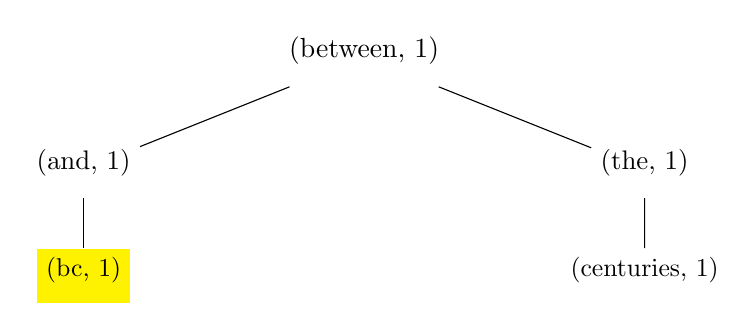
\begin{tikzpicture}
[
    level 1/.style={sibling distance=75mm, scale=1},
    level/.style={sibling distance=35mm, scale=.95},
]
\node [, scale=1.00]
{($\underset{\text{}}{\text{between}}$, 1)} 
    child {node[, scale=0.97]
{($\underset{\text{}}{\text{and}}$, 1)} 
    child {node[fill=yellow, scale=0.93]
{($\underset{\text{}}{\text{bc}}$, 1)} 
}}    child {node[, scale=0.97]
{($\underset{\text{}}{\text{the}}$, 1)} 
    child {node[, scale=0.93]
{($\underset{\text{}}{\text{centuries}}$, 1)} 
}};
\end{tikzpicture}
}
\end{center}

\end{tcolorbox}\section{« the »}
\begin{tcolorbox}[arc=5pt, colback=white!0, colframe=orange!50!black]
\infbox{
Insertion de \textbf{« the »}
}
\begin{center}
\tbox{
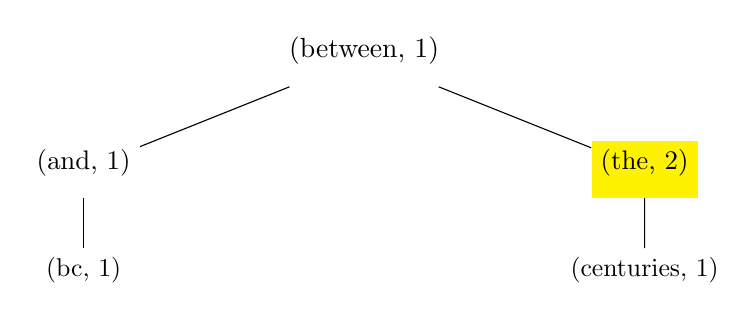
\begin{tikzpicture}
[
    level 1/.style={sibling distance=75mm, scale=1},
    level/.style={sibling distance=35mm, scale=.95},
]
\node [, scale=1.00]
{($\underset{\text{}}{\text{between}}$, 1)} 
    child {node[, scale=0.97]
{($\underset{\text{}}{\text{and}}$, 1)} 
    child {node[, scale=0.93]
{($\underset{\text{}}{\text{bc}}$, 1)} 
}}    child {node[fill=yellow, scale=0.97]
{($\underset{\text{}}{\text{the}}$, 2)} 
    child {node[, scale=0.93]
{($\underset{\text{}}{\text{centuries}}$, 1)} 
}};
\end{tikzpicture}
}
\end{center}

\end{tcolorbox}
\section{« hittites »}
\begin{tcolorbox}[arc=5pt, colback=white!0, colframe=orange!50!black]
\infbox{
Insertion de \textbf{« hittites »}
}
\begin{center}
\tbox{
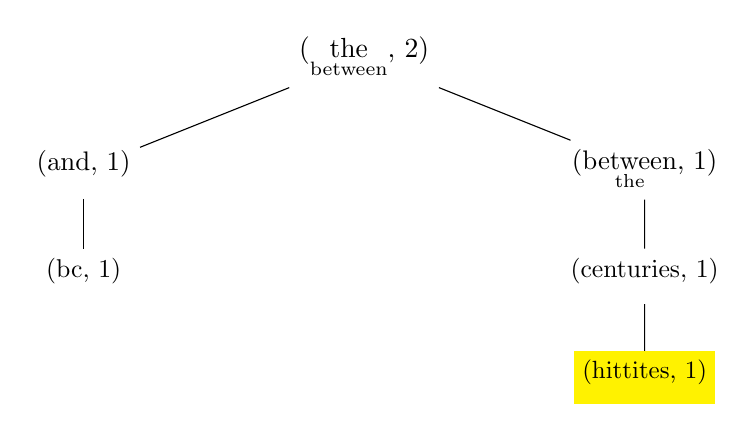
\begin{tikzpicture}
[
    level 1/.style={sibling distance=75mm, scale=1},
    level/.style={sibling distance=35mm, scale=.95},
]
\node [, scale=1.00]
{($\underset{\text{between}}{\text{the}}$, 2)} 
    child {node[, scale=0.97]
{($\underset{\text{}}{\text{and}}$, 1)} 
    child {node[, scale=0.93]
{($\underset{\text{}}{\text{bc}}$, 1)} 
}}    child {node[, scale=0.97]
{($\underset{\text{the}}{\text{between}}$, 1)} 
    child {node[, scale=0.93]
{($\underset{\text{}}{\text{centuries}}$, 1)} 
    child {node[fill=yellow, scale=0.90]
{($\underset{\text{}}{\text{hittites}}$, 1)} 
}}};
\end{tikzpicture}
}
\end{center}

\end{tcolorbox}\section{« were »}
\begin{tcolorbox}[arc=5pt, colback=white!0, colframe=orange!50!black]
\infbox{
Insertion de \textbf{« were »}
}
\begin{center}
\tbox{
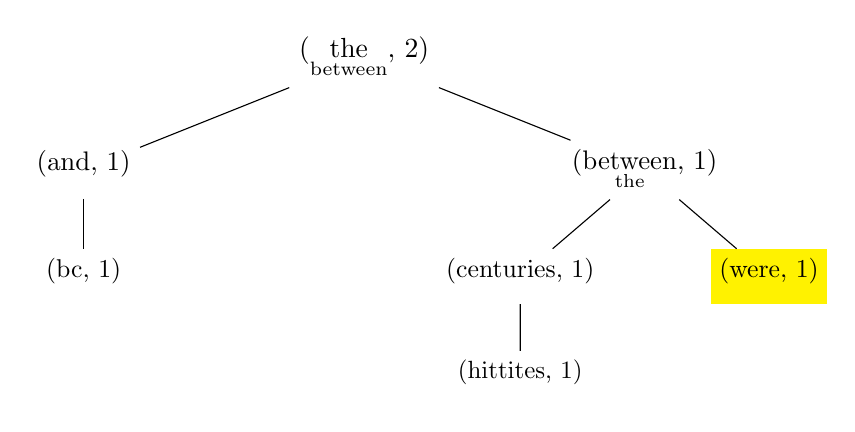
\begin{tikzpicture}
[
    level 1/.style={sibling distance=75mm, scale=1},
    level/.style={sibling distance=35mm, scale=.95},
]
\node [, scale=1.00]
{($\underset{\text{between}}{\text{the}}$, 2)} 
    child {node[, scale=0.97]
{($\underset{\text{}}{\text{and}}$, 1)} 
    child {node[, scale=0.93]
{($\underset{\text{}}{\text{bc}}$, 1)} 
}}    child {node[, scale=0.97]
{($\underset{\text{the}}{\text{between}}$, 1)} 
    child {node[, scale=0.93]
{($\underset{\text{}}{\text{centuries}}$, 1)} 
    child {node[, scale=0.90]
{($\underset{\text{}}{\text{hittites}}$, 1)} 
}}    child {node[fill=yellow, scale=0.93]
{($\underset{\text{}}{\text{were}}$, 1)} 
}};
\end{tikzpicture}
}
\end{center}

\end{tcolorbox}\section{« one »}
\begin{tcolorbox}[arc=5pt, colback=white!0, colframe=orange!50!black]
\infbox{
Insertion de \textbf{« one »}
}
\begin{center}
\tbox{
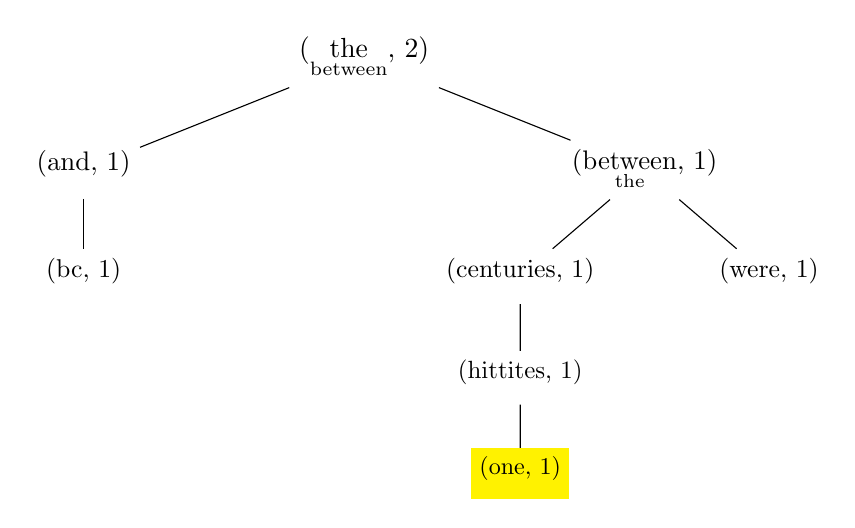
\begin{tikzpicture}
[
    level 1/.style={sibling distance=75mm, scale=1},
    level/.style={sibling distance=35mm, scale=.95},
]
\node [, scale=1.00]
{($\underset{\text{between}}{\text{the}}$, 2)} 
    child {node[, scale=0.97]
{($\underset{\text{}}{\text{and}}$, 1)} 
    child {node[, scale=0.93]
{($\underset{\text{}}{\text{bc}}$, 1)} 
}}    child {node[, scale=0.97]
{($\underset{\text{the}}{\text{between}}$, 1)} 
    child {node[, scale=0.93]
{($\underset{\text{}}{\text{centuries}}$, 1)} 
    child {node[, scale=0.90]
{($\underset{\text{}}{\text{hittites}}$, 1)} 
    child {node[fill=yellow, scale=0.87]
{($\underset{\text{}}{\text{one}}$, 1)} 
}}}    child {node[, scale=0.93]
{($\underset{\text{}}{\text{were}}$, 1)} 
}};
\end{tikzpicture}
}
\end{center}

\end{tcolorbox}\section{« of »}
\begin{tcolorbox}[arc=5pt, colback=white!0, colframe=orange!50!black]
\infbox{
Insertion de \textbf{« of »}
}
\begin{center}
\tbox{
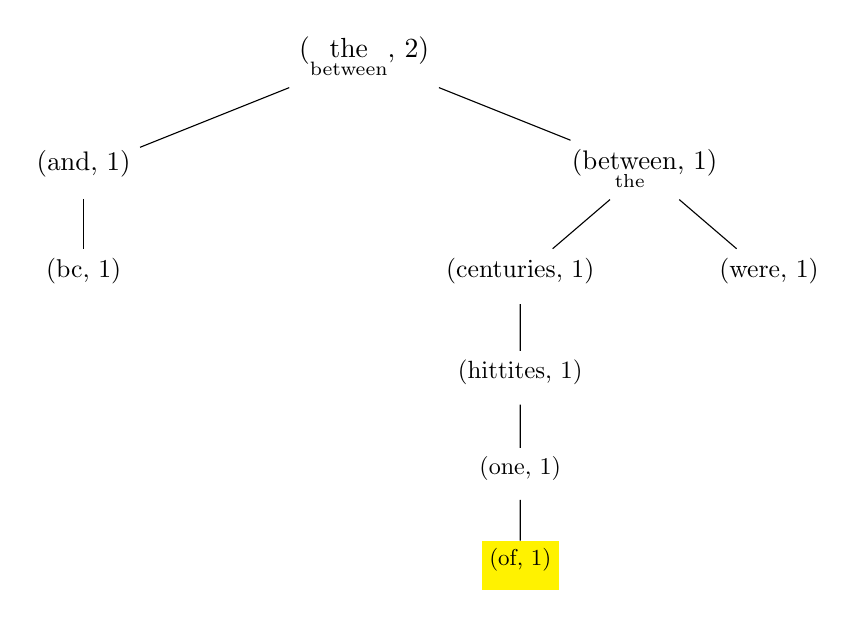
\begin{tikzpicture}
[
    level 1/.style={sibling distance=75mm, scale=1},
    level/.style={sibling distance=35mm, scale=.95},
]
\node [, scale=1.00]
{($\underset{\text{between}}{\text{the}}$, 2)} 
    child {node[, scale=0.97]
{($\underset{\text{}}{\text{and}}$, 1)} 
    child {node[, scale=0.93]
{($\underset{\text{}}{\text{bc}}$, 1)} 
}}    child {node[, scale=0.97]
{($\underset{\text{the}}{\text{between}}$, 1)} 
    child {node[, scale=0.93]
{($\underset{\text{}}{\text{centuries}}$, 1)} 
    child {node[, scale=0.90]
{($\underset{\text{}}{\text{hittites}}$, 1)} 
    child {node[, scale=0.87]
{($\underset{\text{}}{\text{one}}$, 1)} 
    child {node[fill=yellow, scale=0.83]
{($\underset{\text{}}{\text{of}}$, 1)} 
}}}}    child {node[, scale=0.93]
{($\underset{\text{}}{\text{were}}$, 1)} 
}};
\end{tikzpicture}
}
\end{center}

\end{tcolorbox}\section{« the »}
\begin{tcolorbox}[arc=5pt, colback=white!0, colframe=orange!50!black]
\infbox{
Insertion de \textbf{« the »}
}
\begin{center}
\tbox{
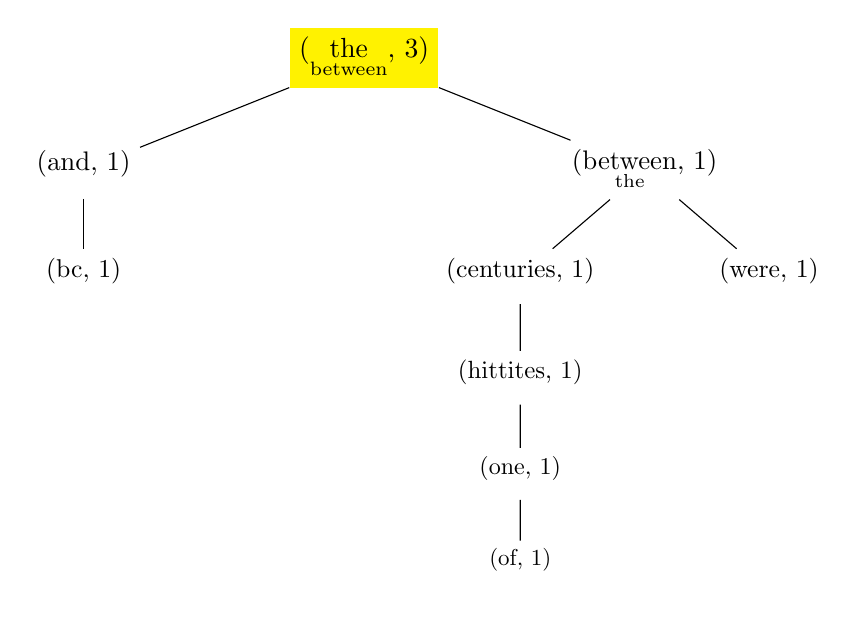
\begin{tikzpicture}
[
    level 1/.style={sibling distance=75mm, scale=1},
    level/.style={sibling distance=35mm, scale=.95},
]
\node [fill=yellow, scale=1.00]
{($\underset{\text{between}}{\text{the}}$, 3)} 
    child {node[, scale=0.97]
{($\underset{\text{}}{\text{and}}$, 1)} 
    child {node[, scale=0.93]
{($\underset{\text{}}{\text{bc}}$, 1)} 
}}    child {node[, scale=0.97]
{($\underset{\text{the}}{\text{between}}$, 1)} 
    child {node[, scale=0.93]
{($\underset{\text{}}{\text{centuries}}$, 1)} 
    child {node[, scale=0.90]
{($\underset{\text{}}{\text{hittites}}$, 1)} 
    child {node[, scale=0.87]
{($\underset{\text{}}{\text{one}}$, 1)} 
    child {node[, scale=0.83]
{($\underset{\text{}}{\text{of}}$, 1)} 
}}}}    child {node[, scale=0.93]
{($\underset{\text{}}{\text{were}}$, 1)} 
}};
\end{tikzpicture}
}
\end{center}

\end{tcolorbox}
\section{« dominant »}
\begin{tcolorbox}[arc=5pt, colback=white!0, colframe=orange!50!black]
\infbox{
Insertion de \textbf{« dominant »}
}
\begin{center}
\tbox{
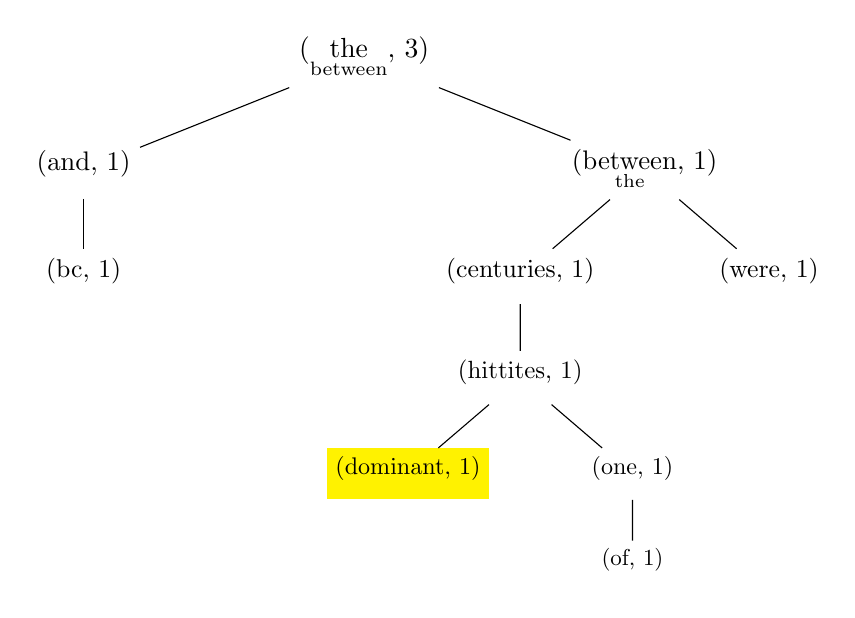
\begin{tikzpicture}
[
    level 1/.style={sibling distance=75mm, scale=1},
    level/.style={sibling distance=35mm, scale=.95},
]
\node [, scale=1.00]
{($\underset{\text{between}}{\text{the}}$, 3)} 
    child {node[, scale=0.97]
{($\underset{\text{}}{\text{and}}$, 1)} 
    child {node[, scale=0.93]
{($\underset{\text{}}{\text{bc}}$, 1)} 
}}    child {node[, scale=0.97]
{($\underset{\text{the}}{\text{between}}$, 1)} 
    child {node[, scale=0.93]
{($\underset{\text{}}{\text{centuries}}$, 1)} 
    child {node[, scale=0.90]
{($\underset{\text{}}{\text{hittites}}$, 1)} 
    child {node[fill=yellow, scale=0.87]
{($\underset{\text{}}{\text{dominant}}$, 1)} 
}    child {node[, scale=0.87]
{($\underset{\text{}}{\text{one}}$, 1)} 
    child {node[, scale=0.83]
{($\underset{\text{}}{\text{of}}$, 1)} 
}}}}    child {node[, scale=0.93]
{($\underset{\text{}}{\text{were}}$, 1)} 
}};
\end{tikzpicture}
}
\end{center}

\end{tcolorbox}\section{« powers »}
\begin{tcolorbox}[arc=5pt, colback=white!0, colframe=orange!50!black]
\infbox{
Insertion de \textbf{« powers »}
}
\begin{center}
\tbox{
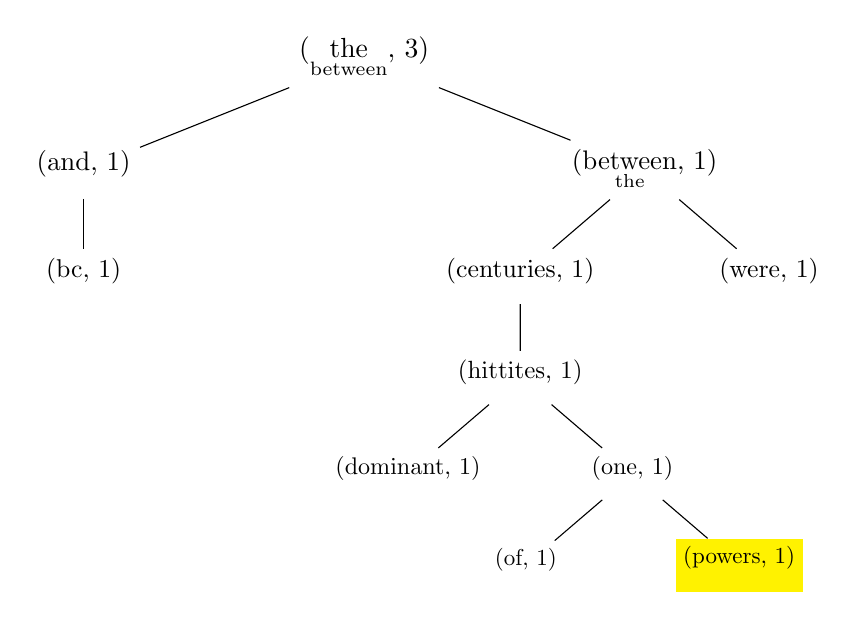
\begin{tikzpicture}
[
    level 1/.style={sibling distance=75mm, scale=1},
    level/.style={sibling distance=35mm, scale=.95},
]
\node [, scale=1.00]
{($\underset{\text{between}}{\text{the}}$, 3)} 
    child {node[, scale=0.97]
{($\underset{\text{}}{\text{and}}$, 1)} 
    child {node[, scale=0.93]
{($\underset{\text{}}{\text{bc}}$, 1)} 
}}    child {node[, scale=0.97]
{($\underset{\text{the}}{\text{between}}$, 1)} 
    child {node[, scale=0.93]
{($\underset{\text{}}{\text{centuries}}$, 1)} 
    child {node[, scale=0.90]
{($\underset{\text{}}{\text{hittites}}$, 1)} 
    child {node[, scale=0.87]
{($\underset{\text{}}{\text{dominant}}$, 1)} 
}    child {node[, scale=0.87]
{($\underset{\text{}}{\text{one}}$, 1)} 
    child {node[, scale=0.83]
{($\underset{\text{}}{\text{of}}$, 1)} 
}    child {node[fill=yellow, scale=0.83]
{($\underset{\text{}}{\text{powers}}$, 1)} 
}}}}    child {node[, scale=0.93]
{($\underset{\text{}}{\text{were}}$, 1)} 
}};
\end{tikzpicture}
}
\end{center}

\end{tcolorbox}\section{« of »}
\begin{tcolorbox}[arc=5pt, colback=white!0, colframe=orange!50!black]
\infbox{
Insertion de \textbf{« of »}
}
\begin{center}
\tbox{
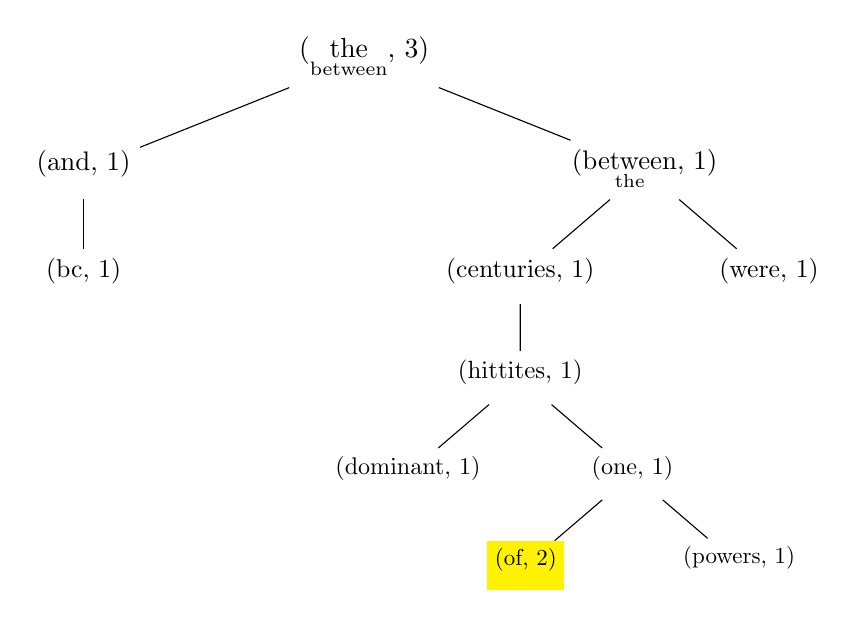
\begin{tikzpicture}
[
    level 1/.style={sibling distance=75mm, scale=1},
    level/.style={sibling distance=35mm, scale=.95},
]
\node [, scale=1.00]
{($\underset{\text{between}}{\text{the}}$, 3)} 
    child {node[, scale=0.97]
{($\underset{\text{}}{\text{and}}$, 1)} 
    child {node[, scale=0.93]
{($\underset{\text{}}{\text{bc}}$, 1)} 
}}    child {node[, scale=0.97]
{($\underset{\text{the}}{\text{between}}$, 1)} 
    child {node[, scale=0.93]
{($\underset{\text{}}{\text{centuries}}$, 1)} 
    child {node[, scale=0.90]
{($\underset{\text{}}{\text{hittites}}$, 1)} 
    child {node[, scale=0.87]
{($\underset{\text{}}{\text{dominant}}$, 1)} 
}    child {node[, scale=0.87]
{($\underset{\text{}}{\text{one}}$, 1)} 
    child {node[fill=yellow, scale=0.83]
{($\underset{\text{}}{\text{of}}$, 2)} 
}    child {node[, scale=0.83]
{($\underset{\text{}}{\text{powers}}$, 1)} 
}}}}    child {node[, scale=0.93]
{($\underset{\text{}}{\text{were}}$, 1)} 
}};
\end{tikzpicture}
}
\end{center}

\end{tcolorbox}
\section{« the »}
\begin{tcolorbox}[arc=5pt, colback=white!0, colframe=orange!50!black]
\infbox{
Insertion de \textbf{« the »}
}
\begin{center}
\tbox{
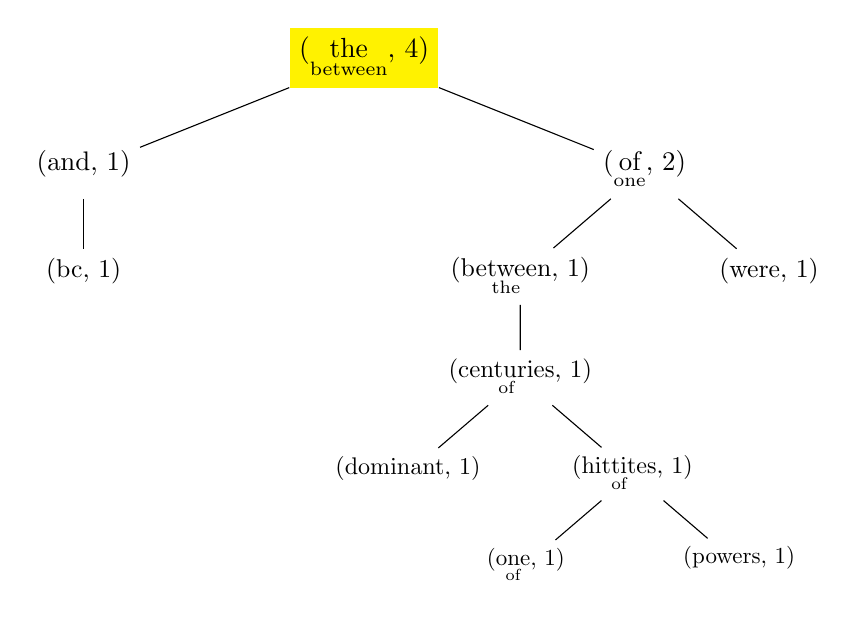
\begin{tikzpicture}
[
    level 1/.style={sibling distance=75mm, scale=1},
    level/.style={sibling distance=35mm, scale=.95},
]
\node [fill=yellow, scale=1.00]
{($\underset{\text{between}}{\text{the}}$, 4)} 
    child {node[, scale=0.97]
{($\underset{\text{}}{\text{and}}$, 1)} 
    child {node[, scale=0.93]
{($\underset{\text{}}{\text{bc}}$, 1)} 
}}    child {node[, scale=0.97]
{($\underset{\text{one}}{\text{of}}$, 2)} 
    child {node[, scale=0.93]
{($\underset{\text{the}}{\text{between}}$, 1)} 
    child {node[, scale=0.90]
{($\underset{\text{of}}{\text{centuries}}$, 1)} 
    child {node[, scale=0.87]
{($\underset{\text{}}{\text{dominant}}$, 1)} 
}    child {node[, scale=0.87]
{($\underset{\text{of}}{\text{hittites}}$, 1)} 
    child {node[, scale=0.83]
{($\underset{\text{of}}{\text{one}}$, 1)} 
}    child {node[, scale=0.83]
{($\underset{\text{}}{\text{powers}}$, 1)} 
}}}}    child {node[, scale=0.93]
{($\underset{\text{}}{\text{were}}$, 1)} 
}};
\end{tikzpicture}
}
\end{center}

\end{tcolorbox}
\section{« near »}
\begin{tcolorbox}[arc=5pt, colback=white!0, colframe=orange!50!black]
\infbox{
Insertion de \textbf{« near »}
}
\begin{center}
\tbox{
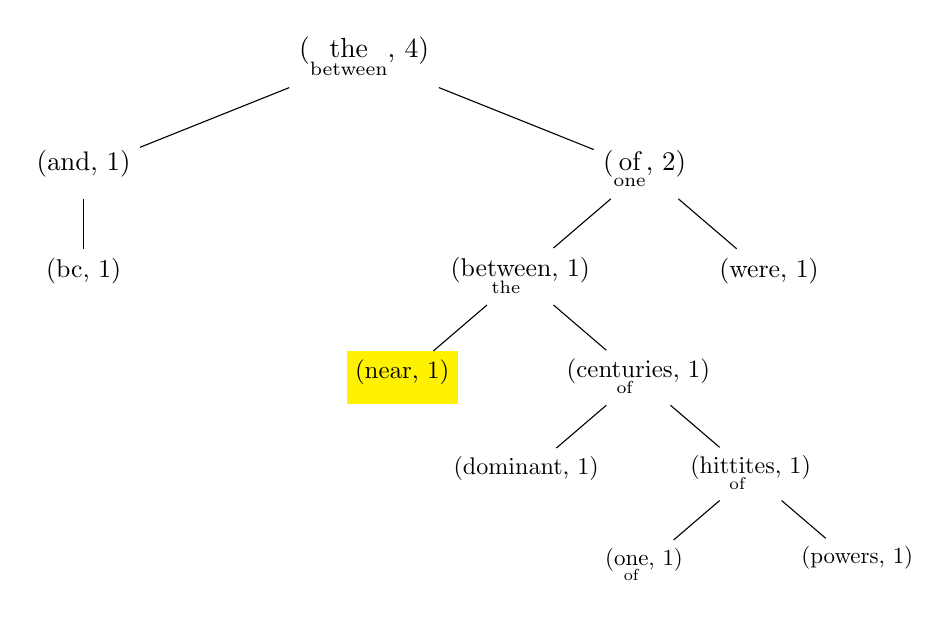
\begin{tikzpicture}
[
    level 1/.style={sibling distance=75mm, scale=1},
    level/.style={sibling distance=35mm, scale=.95},
]
\node [, scale=1.00]
{($\underset{\text{between}}{\text{the}}$, 4)} 
    child {node[, scale=0.97]
{($\underset{\text{}}{\text{and}}$, 1)} 
    child {node[, scale=0.93]
{($\underset{\text{}}{\text{bc}}$, 1)} 
}}    child {node[, scale=0.97]
{($\underset{\text{one}}{\text{of}}$, 2)} 
    child {node[, scale=0.93]
{($\underset{\text{the}}{\text{between}}$, 1)} 
    child {node[fill=yellow, scale=0.90]
{($\underset{\text{}}{\text{near}}$, 1)} 
}    child {node[, scale=0.90]
{($\underset{\text{of}}{\text{centuries}}$, 1)} 
    child {node[, scale=0.87]
{($\underset{\text{}}{\text{dominant}}$, 1)} 
}    child {node[, scale=0.87]
{($\underset{\text{of}}{\text{hittites}}$, 1)} 
    child {node[, scale=0.83]
{($\underset{\text{of}}{\text{one}}$, 1)} 
}    child {node[, scale=0.83]
{($\underset{\text{}}{\text{powers}}$, 1)} 
}}}}    child {node[, scale=0.93]
{($\underset{\text{}}{\text{were}}$, 1)} 
}};
\end{tikzpicture}
}
\end{center}

\end{tcolorbox}\section{« east »}
\begin{tcolorbox}[arc=5pt, colback=white!0, colframe=orange!50!black]
\infbox{
Insertion de \textbf{« east »}
}
\begin{center}
\tbox{
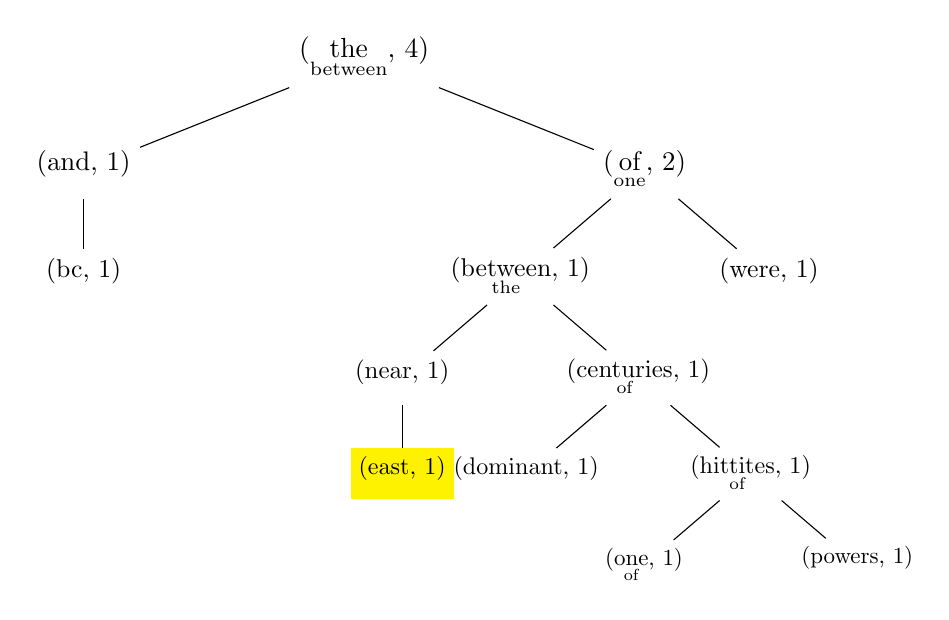
\begin{tikzpicture}
[
    level 1/.style={sibling distance=75mm, scale=1},
    level/.style={sibling distance=35mm, scale=.95},
]
\node [, scale=1.00]
{($\underset{\text{between}}{\text{the}}$, 4)} 
    child {node[, scale=0.97]
{($\underset{\text{}}{\text{and}}$, 1)} 
    child {node[, scale=0.93]
{($\underset{\text{}}{\text{bc}}$, 1)} 
}}    child {node[, scale=0.97]
{($\underset{\text{one}}{\text{of}}$, 2)} 
    child {node[, scale=0.93]
{($\underset{\text{the}}{\text{between}}$, 1)} 
    child {node[, scale=0.90]
{($\underset{\text{}}{\text{near}}$, 1)} 
    child {node[fill=yellow, scale=0.87]
{($\underset{\text{}}{\text{east}}$, 1)} 
}}    child {node[, scale=0.90]
{($\underset{\text{of}}{\text{centuries}}$, 1)} 
    child {node[, scale=0.87]
{($\underset{\text{}}{\text{dominant}}$, 1)} 
}    child {node[, scale=0.87]
{($\underset{\text{of}}{\text{hittites}}$, 1)} 
    child {node[, scale=0.83]
{($\underset{\text{of}}{\text{one}}$, 1)} 
}    child {node[, scale=0.83]
{($\underset{\text{}}{\text{powers}}$, 1)} 
}}}}    child {node[, scale=0.93]
{($\underset{\text{}}{\text{were}}$, 1)} 
}};
\end{tikzpicture}
}
\end{center}

\end{tcolorbox}\section{« coming »}
\begin{tcolorbox}[arc=5pt, colback=white!0, colframe=orange!50!black]
\infbox{
Insertion de \textbf{« coming »}
}
\begin{center}
\tbox{
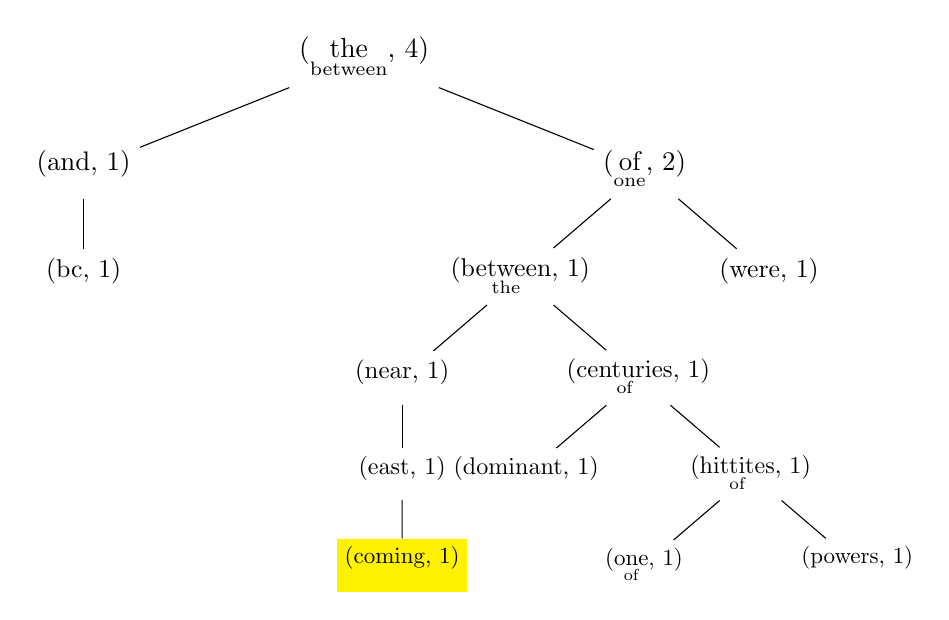
\begin{tikzpicture}
[
    level 1/.style={sibling distance=75mm, scale=1},
    level/.style={sibling distance=35mm, scale=.95},
]
\node [, scale=1.00]
{($\underset{\text{between}}{\text{the}}$, 4)} 
    child {node[, scale=0.97]
{($\underset{\text{}}{\text{and}}$, 1)} 
    child {node[, scale=0.93]
{($\underset{\text{}}{\text{bc}}$, 1)} 
}}    child {node[, scale=0.97]
{($\underset{\text{one}}{\text{of}}$, 2)} 
    child {node[, scale=0.93]
{($\underset{\text{the}}{\text{between}}$, 1)} 
    child {node[, scale=0.90]
{($\underset{\text{}}{\text{near}}$, 1)} 
    child {node[, scale=0.87]
{($\underset{\text{}}{\text{east}}$, 1)} 
    child {node[fill=yellow, scale=0.83]
{($\underset{\text{}}{\text{coming}}$, 1)} 
}}}    child {node[, scale=0.90]
{($\underset{\text{of}}{\text{centuries}}$, 1)} 
    child {node[, scale=0.87]
{($\underset{\text{}}{\text{dominant}}$, 1)} 
}    child {node[, scale=0.87]
{($\underset{\text{of}}{\text{hittites}}$, 1)} 
    child {node[, scale=0.83]
{($\underset{\text{of}}{\text{one}}$, 1)} 
}    child {node[, scale=0.83]
{($\underset{\text{}}{\text{powers}}$, 1)} 
}}}}    child {node[, scale=0.93]
{($\underset{\text{}}{\text{were}}$, 1)} 
}};
\end{tikzpicture}
}
\end{center}

\end{tcolorbox}\section{« into »}
\begin{tcolorbox}[arc=5pt, colback=white!0, colframe=orange!50!black]
\infbox{
Insertion de \textbf{« into »}
}
\begin{center}
\tbox{
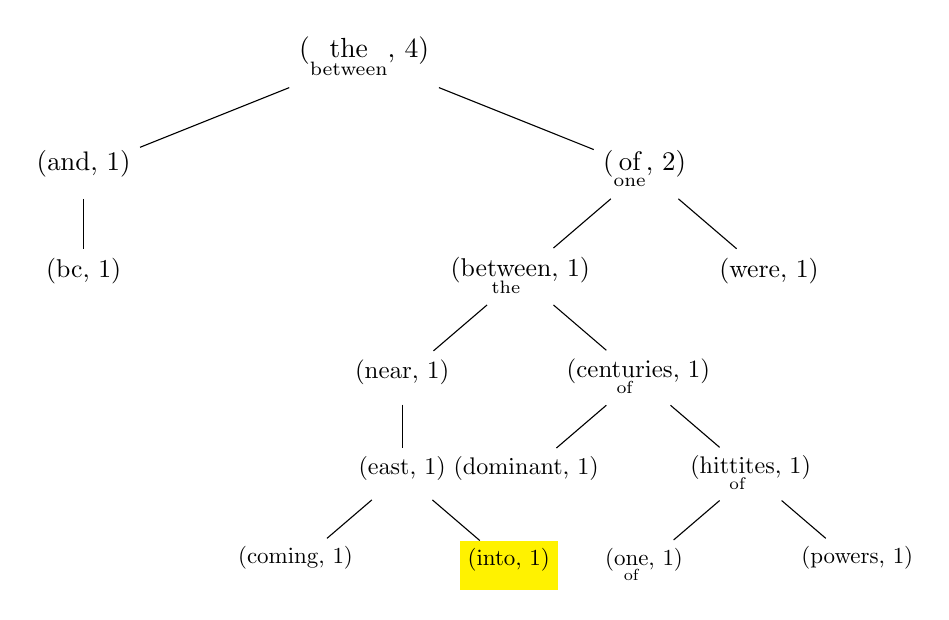
\begin{tikzpicture}
[
    level 1/.style={sibling distance=75mm, scale=1},
    level/.style={sibling distance=35mm, scale=.95},
]
\node [, scale=1.00]
{($\underset{\text{between}}{\text{the}}$, 4)} 
    child {node[, scale=0.97]
{($\underset{\text{}}{\text{and}}$, 1)} 
    child {node[, scale=0.93]
{($\underset{\text{}}{\text{bc}}$, 1)} 
}}    child {node[, scale=0.97]
{($\underset{\text{one}}{\text{of}}$, 2)} 
    child {node[, scale=0.93]
{($\underset{\text{the}}{\text{between}}$, 1)} 
    child {node[, scale=0.90]
{($\underset{\text{}}{\text{near}}$, 1)} 
    child {node[, scale=0.87]
{($\underset{\text{}}{\text{east}}$, 1)} 
    child {node[, scale=0.83]
{($\underset{\text{}}{\text{coming}}$, 1)} 
}    child {node[fill=yellow, scale=0.83]
{($\underset{\text{}}{\text{into}}$, 1)} 
}}}    child {node[, scale=0.90]
{($\underset{\text{of}}{\text{centuries}}$, 1)} 
    child {node[, scale=0.87]
{($\underset{\text{}}{\text{dominant}}$, 1)} 
}    child {node[, scale=0.87]
{($\underset{\text{of}}{\text{hittites}}$, 1)} 
    child {node[, scale=0.83]
{($\underset{\text{of}}{\text{one}}$, 1)} 
}    child {node[, scale=0.83]
{($\underset{\text{}}{\text{powers}}$, 1)} 
}}}}    child {node[, scale=0.93]
{($\underset{\text{}}{\text{were}}$, 1)} 
}};
\end{tikzpicture}
}
\end{center}

\end{tcolorbox}\section{« conflict »}
\begin{tcolorbox}[arc=5pt, colback=white!0, colframe=orange!50!black]
\infbox{
Insertion de \textbf{« conflict »}
}
\begin{center}
\tbox{
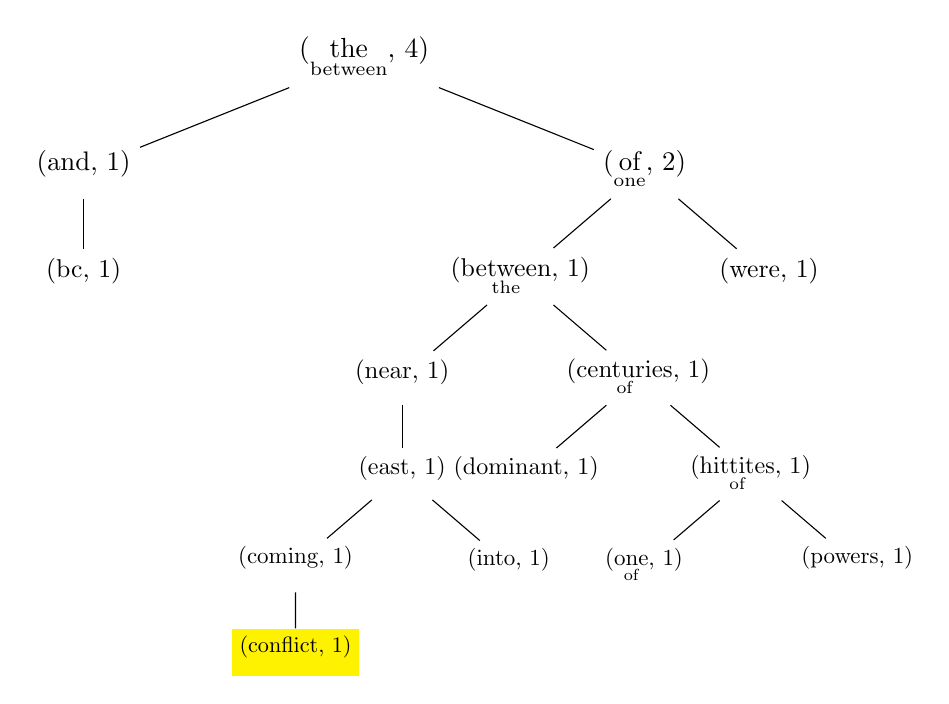
\begin{tikzpicture}
[
    level 1/.style={sibling distance=75mm, scale=1},
    level/.style={sibling distance=35mm, scale=.95},
]
\node [, scale=1.00]
{($\underset{\text{between}}{\text{the}}$, 4)} 
    child {node[, scale=0.97]
{($\underset{\text{}}{\text{and}}$, 1)} 
    child {node[, scale=0.93]
{($\underset{\text{}}{\text{bc}}$, 1)} 
}}    child {node[, scale=0.97]
{($\underset{\text{one}}{\text{of}}$, 2)} 
    child {node[, scale=0.93]
{($\underset{\text{the}}{\text{between}}$, 1)} 
    child {node[, scale=0.90]
{($\underset{\text{}}{\text{near}}$, 1)} 
    child {node[, scale=0.87]
{($\underset{\text{}}{\text{east}}$, 1)} 
    child {node[, scale=0.83]
{($\underset{\text{}}{\text{coming}}$, 1)} 
    child {node[fill=yellow, scale=0.80]
{($\underset{\text{}}{\text{conflict}}$, 1)} 
}}    child {node[, scale=0.83]
{($\underset{\text{}}{\text{into}}$, 1)} 
}}}    child {node[, scale=0.90]
{($\underset{\text{of}}{\text{centuries}}$, 1)} 
    child {node[, scale=0.87]
{($\underset{\text{}}{\text{dominant}}$, 1)} 
}    child {node[, scale=0.87]
{($\underset{\text{of}}{\text{hittites}}$, 1)} 
    child {node[, scale=0.83]
{($\underset{\text{of}}{\text{one}}$, 1)} 
}    child {node[, scale=0.83]
{($\underset{\text{}}{\text{powers}}$, 1)} 
}}}}    child {node[, scale=0.93]
{($\underset{\text{}}{\text{were}}$, 1)} 
}};
\end{tikzpicture}
}
\end{center}

\end{tcolorbox}\section{« with »}
\begin{tcolorbox}[arc=5pt, colback=white!0, colframe=orange!50!black]
\infbox{
Insertion de \textbf{« with »}
}
\begin{center}
\tbox{
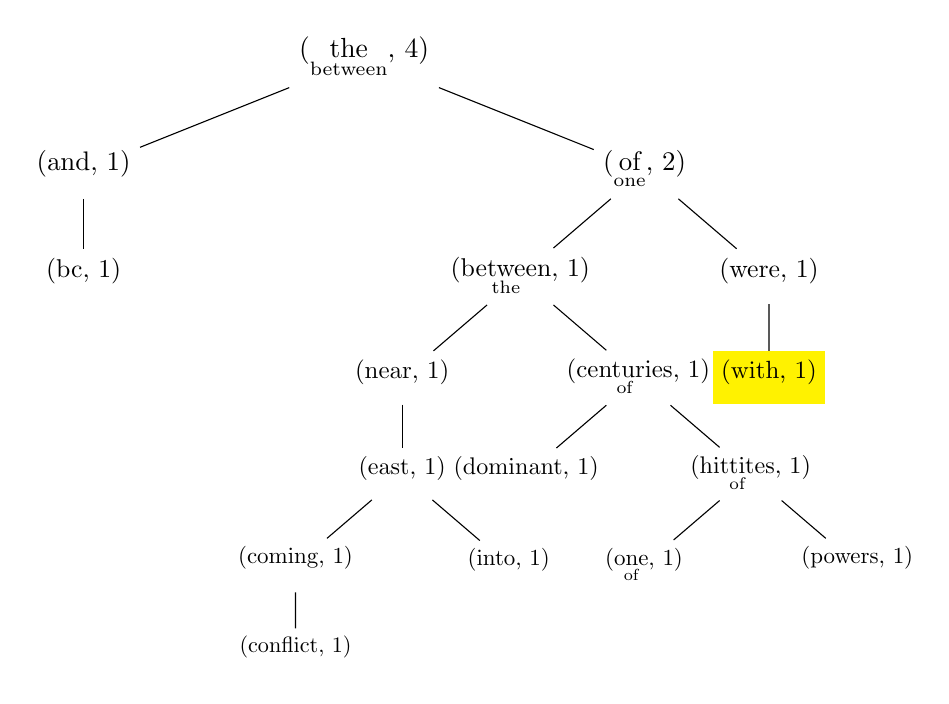
\begin{tikzpicture}
[
    level 1/.style={sibling distance=75mm, scale=1},
    level/.style={sibling distance=35mm, scale=.95},
]
\node [, scale=1.00]
{($\underset{\text{between}}{\text{the}}$, 4)} 
    child {node[, scale=0.97]
{($\underset{\text{}}{\text{and}}$, 1)} 
    child {node[, scale=0.93]
{($\underset{\text{}}{\text{bc}}$, 1)} 
}}    child {node[, scale=0.97]
{($\underset{\text{one}}{\text{of}}$, 2)} 
    child {node[, scale=0.93]
{($\underset{\text{the}}{\text{between}}$, 1)} 
    child {node[, scale=0.90]
{($\underset{\text{}}{\text{near}}$, 1)} 
    child {node[, scale=0.87]
{($\underset{\text{}}{\text{east}}$, 1)} 
    child {node[, scale=0.83]
{($\underset{\text{}}{\text{coming}}$, 1)} 
    child {node[, scale=0.80]
{($\underset{\text{}}{\text{conflict}}$, 1)} 
}}    child {node[, scale=0.83]
{($\underset{\text{}}{\text{into}}$, 1)} 
}}}    child {node[, scale=0.90]
{($\underset{\text{of}}{\text{centuries}}$, 1)} 
    child {node[, scale=0.87]
{($\underset{\text{}}{\text{dominant}}$, 1)} 
}    child {node[, scale=0.87]
{($\underset{\text{of}}{\text{hittites}}$, 1)} 
    child {node[, scale=0.83]
{($\underset{\text{of}}{\text{one}}$, 1)} 
}    child {node[, scale=0.83]
{($\underset{\text{}}{\text{powers}}$, 1)} 
}}}}    child {node[, scale=0.93]
{($\underset{\text{}}{\text{were}}$, 1)} 
    child {node[fill=yellow, scale=0.90]
{($\underset{\text{}}{\text{with}}$, 1)} 
}}};
\end{tikzpicture}
}
\end{center}

\end{tcolorbox}\section{« the »}
\begin{tcolorbox}[arc=5pt, colback=white!0, colframe=orange!50!black]
\infbox{
Insertion de \textbf{« the »}
}
\begin{center}
\tbox{
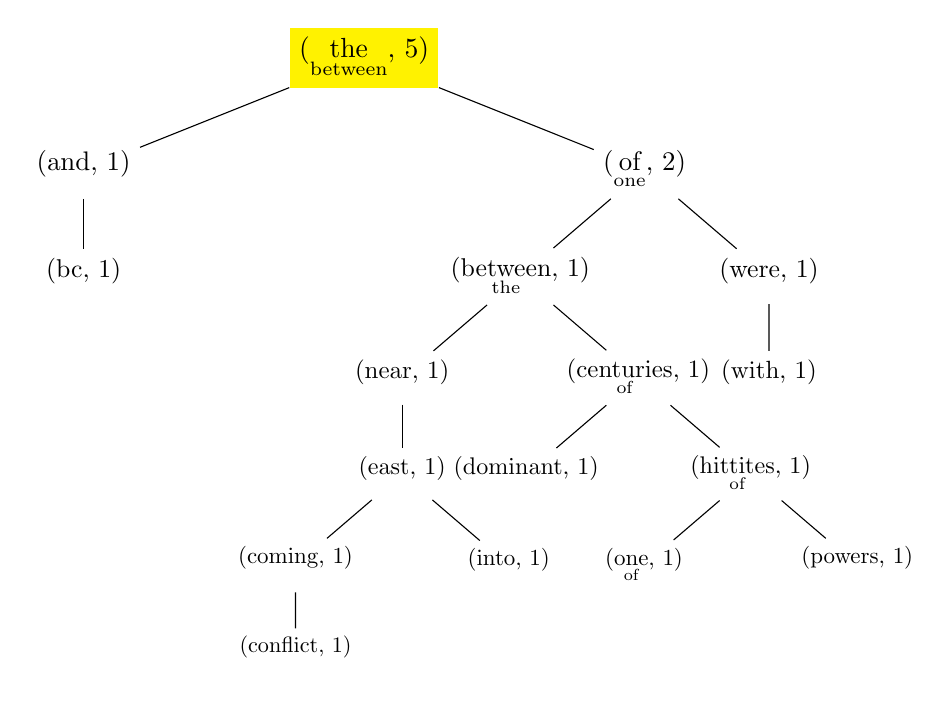
\begin{tikzpicture}
[
    level 1/.style={sibling distance=75mm, scale=1},
    level/.style={sibling distance=35mm, scale=.95},
]
\node [fill=yellow, scale=1.00]
{($\underset{\text{between}}{\text{the}}$, 5)} 
    child {node[, scale=0.97]
{($\underset{\text{}}{\text{and}}$, 1)} 
    child {node[, scale=0.93]
{($\underset{\text{}}{\text{bc}}$, 1)} 
}}    child {node[, scale=0.97]
{($\underset{\text{one}}{\text{of}}$, 2)} 
    child {node[, scale=0.93]
{($\underset{\text{the}}{\text{between}}$, 1)} 
    child {node[, scale=0.90]
{($\underset{\text{}}{\text{near}}$, 1)} 
    child {node[, scale=0.87]
{($\underset{\text{}}{\text{east}}$, 1)} 
    child {node[, scale=0.83]
{($\underset{\text{}}{\text{coming}}$, 1)} 
    child {node[, scale=0.80]
{($\underset{\text{}}{\text{conflict}}$, 1)} 
}}    child {node[, scale=0.83]
{($\underset{\text{}}{\text{into}}$, 1)} 
}}}    child {node[, scale=0.90]
{($\underset{\text{of}}{\text{centuries}}$, 1)} 
    child {node[, scale=0.87]
{($\underset{\text{}}{\text{dominant}}$, 1)} 
}    child {node[, scale=0.87]
{($\underset{\text{of}}{\text{hittites}}$, 1)} 
    child {node[, scale=0.83]
{($\underset{\text{of}}{\text{one}}$, 1)} 
}    child {node[, scale=0.83]
{($\underset{\text{}}{\text{powers}}$, 1)} 
}}}}    child {node[, scale=0.93]
{($\underset{\text{}}{\text{were}}$, 1)} 
    child {node[, scale=0.90]
{($\underset{\text{}}{\text{with}}$, 1)} 
}}};
\end{tikzpicture}
}
\end{center}

\end{tcolorbox}
\section{« new »}
\begin{tcolorbox}[arc=5pt, colback=white!0, colframe=orange!50!black]
\infbox{
Insertion de \textbf{« new »}
}
\begin{center}
\tbox{
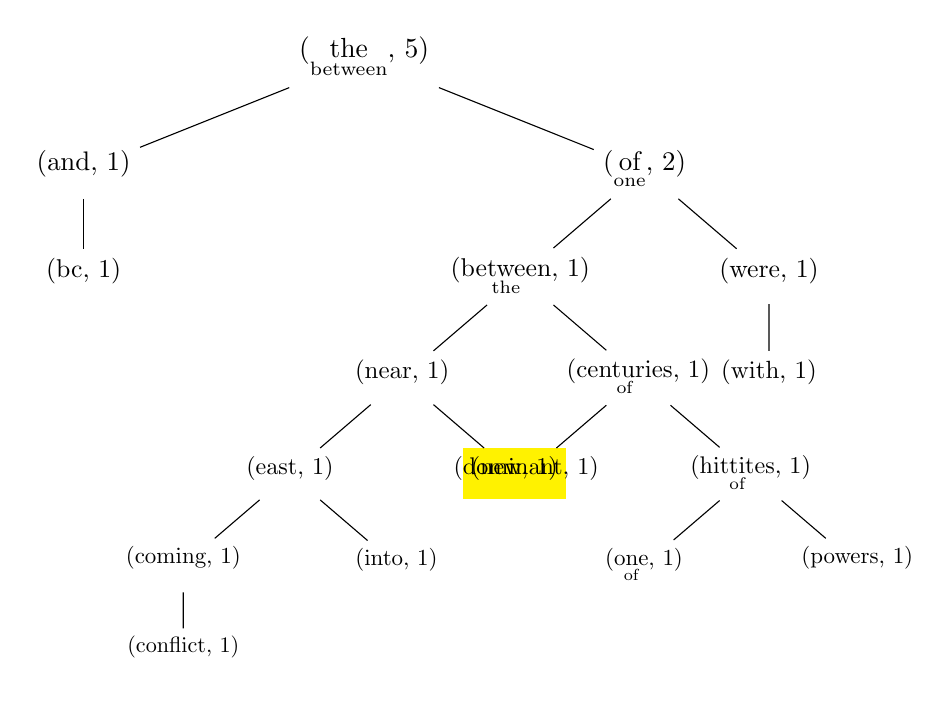
\begin{tikzpicture}
[
    level 1/.style={sibling distance=75mm, scale=1},
    level/.style={sibling distance=35mm, scale=.95},
]
\node [, scale=1.00]
{($\underset{\text{between}}{\text{the}}$, 5)} 
    child {node[, scale=0.97]
{($\underset{\text{}}{\text{and}}$, 1)} 
    child {node[, scale=0.93]
{($\underset{\text{}}{\text{bc}}$, 1)} 
}}    child {node[, scale=0.97]
{($\underset{\text{one}}{\text{of}}$, 2)} 
    child {node[, scale=0.93]
{($\underset{\text{the}}{\text{between}}$, 1)} 
    child {node[, scale=0.90]
{($\underset{\text{}}{\text{near}}$, 1)} 
    child {node[, scale=0.87]
{($\underset{\text{}}{\text{east}}$, 1)} 
    child {node[, scale=0.83]
{($\underset{\text{}}{\text{coming}}$, 1)} 
    child {node[, scale=0.80]
{($\underset{\text{}}{\text{conflict}}$, 1)} 
}}    child {node[, scale=0.83]
{($\underset{\text{}}{\text{into}}$, 1)} 
}}    child {node[fill=yellow, scale=0.87]
{($\underset{\text{}}{\text{new}}$, 1)} 
}}    child {node[, scale=0.90]
{($\underset{\text{of}}{\text{centuries}}$, 1)} 
    child {node[, scale=0.87]
{($\underset{\text{}}{\text{dominant}}$, 1)} 
}    child {node[, scale=0.87]
{($\underset{\text{of}}{\text{hittites}}$, 1)} 
    child {node[, scale=0.83]
{($\underset{\text{of}}{\text{one}}$, 1)} 
}    child {node[, scale=0.83]
{($\underset{\text{}}{\text{powers}}$, 1)} 
}}}}    child {node[, scale=0.93]
{($\underset{\text{}}{\text{were}}$, 1)} 
    child {node[, scale=0.90]
{($\underset{\text{}}{\text{with}}$, 1)} 
}}};
\end{tikzpicture}
}
\end{center}

\end{tcolorbox}\section{« kingdom »}
\begin{tcolorbox}[arc=5pt, colback=white!0, colframe=orange!50!black]
\infbox{
Insertion de \textbf{« kingdom »}
}
\begin{center}
\tbox{
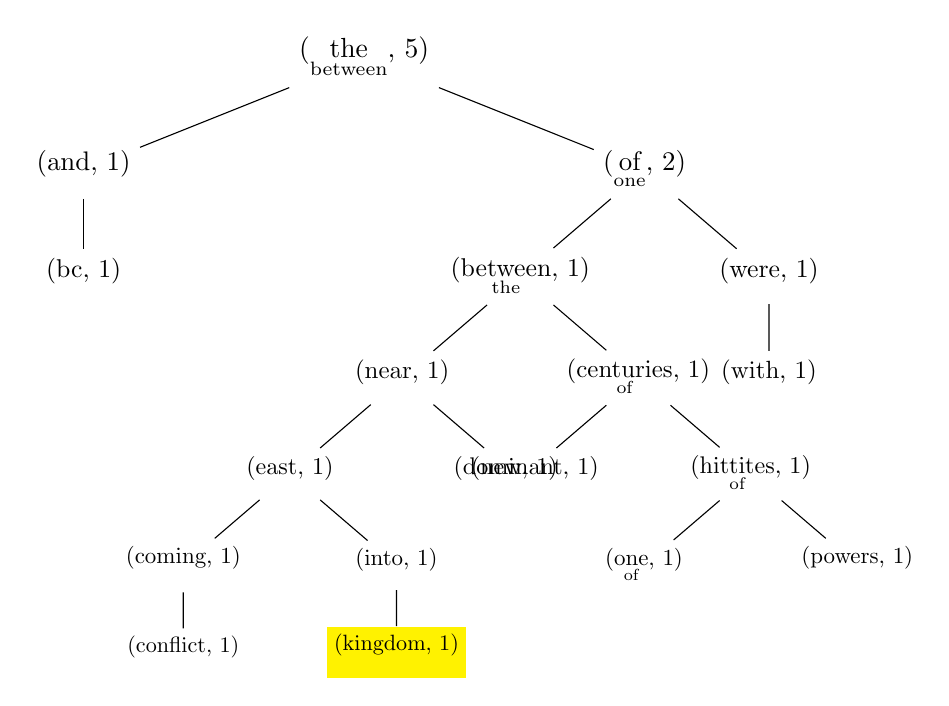
\begin{tikzpicture}
[
    level 1/.style={sibling distance=75mm, scale=1},
    level/.style={sibling distance=35mm, scale=.95},
]
\node [, scale=1.00]
{($\underset{\text{between}}{\text{the}}$, 5)} 
    child {node[, scale=0.97]
{($\underset{\text{}}{\text{and}}$, 1)} 
    child {node[, scale=0.93]
{($\underset{\text{}}{\text{bc}}$, 1)} 
}}    child {node[, scale=0.97]
{($\underset{\text{one}}{\text{of}}$, 2)} 
    child {node[, scale=0.93]
{($\underset{\text{the}}{\text{between}}$, 1)} 
    child {node[, scale=0.90]
{($\underset{\text{}}{\text{near}}$, 1)} 
    child {node[, scale=0.87]
{($\underset{\text{}}{\text{east}}$, 1)} 
    child {node[, scale=0.83]
{($\underset{\text{}}{\text{coming}}$, 1)} 
    child {node[, scale=0.80]
{($\underset{\text{}}{\text{conflict}}$, 1)} 
}}    child {node[, scale=0.83]
{($\underset{\text{}}{\text{into}}$, 1)} 
    child {node[fill=yellow, scale=0.80]
{($\underset{\text{}}{\text{kingdom}}$, 1)} 
}}}    child {node[, scale=0.87]
{($\underset{\text{}}{\text{new}}$, 1)} 
}}    child {node[, scale=0.90]
{($\underset{\text{of}}{\text{centuries}}$, 1)} 
    child {node[, scale=0.87]
{($\underset{\text{}}{\text{dominant}}$, 1)} 
}    child {node[, scale=0.87]
{($\underset{\text{of}}{\text{hittites}}$, 1)} 
    child {node[, scale=0.83]
{($\underset{\text{of}}{\text{one}}$, 1)} 
}    child {node[, scale=0.83]
{($\underset{\text{}}{\text{powers}}$, 1)} 
}}}}    child {node[, scale=0.93]
{($\underset{\text{}}{\text{were}}$, 1)} 
    child {node[, scale=0.90]
{($\underset{\text{}}{\text{with}}$, 1)} 
}}};
\end{tikzpicture}
}
\end{center}

\end{tcolorbox}\section{« of »}
\begin{tcolorbox}[arc=5pt, colback=white!0, colframe=orange!50!black]
\infbox{
Insertion de \textbf{« of »}
}
\begin{center}
\tbox{
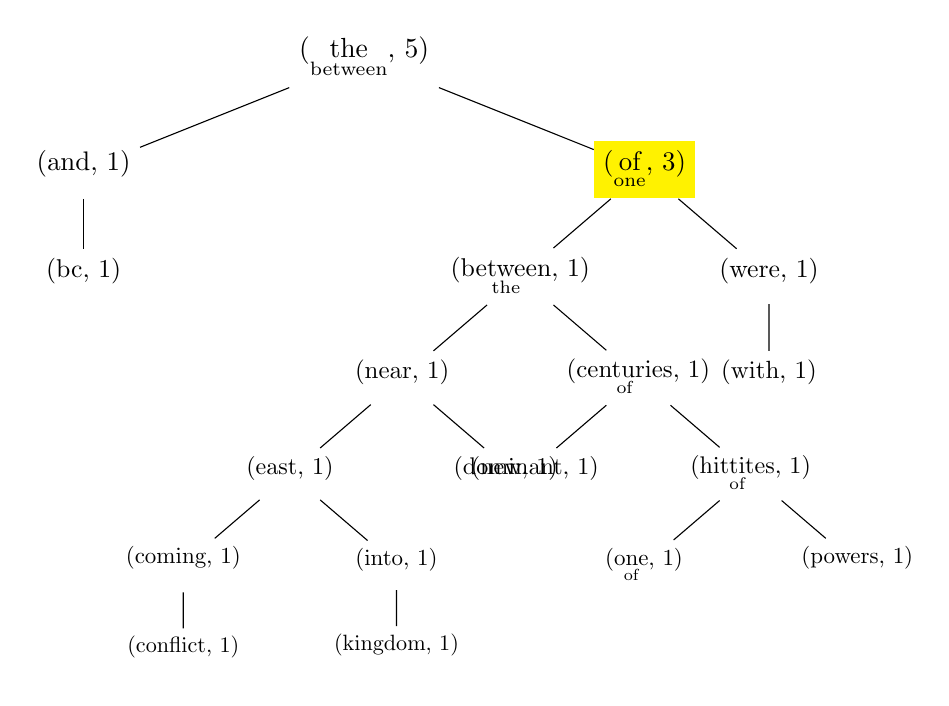
\begin{tikzpicture}
[
    level 1/.style={sibling distance=75mm, scale=1},
    level/.style={sibling distance=35mm, scale=.95},
]
\node [, scale=1.00]
{($\underset{\text{between}}{\text{the}}$, 5)} 
    child {node[, scale=0.97]
{($\underset{\text{}}{\text{and}}$, 1)} 
    child {node[, scale=0.93]
{($\underset{\text{}}{\text{bc}}$, 1)} 
}}    child {node[fill=yellow, scale=0.97]
{($\underset{\text{one}}{\text{of}}$, 3)} 
    child {node[, scale=0.93]
{($\underset{\text{the}}{\text{between}}$, 1)} 
    child {node[, scale=0.90]
{($\underset{\text{}}{\text{near}}$, 1)} 
    child {node[, scale=0.87]
{($\underset{\text{}}{\text{east}}$, 1)} 
    child {node[, scale=0.83]
{($\underset{\text{}}{\text{coming}}$, 1)} 
    child {node[, scale=0.80]
{($\underset{\text{}}{\text{conflict}}$, 1)} 
}}    child {node[, scale=0.83]
{($\underset{\text{}}{\text{into}}$, 1)} 
    child {node[, scale=0.80]
{($\underset{\text{}}{\text{kingdom}}$, 1)} 
}}}    child {node[, scale=0.87]
{($\underset{\text{}}{\text{new}}$, 1)} 
}}    child {node[, scale=0.90]
{($\underset{\text{of}}{\text{centuries}}$, 1)} 
    child {node[, scale=0.87]
{($\underset{\text{}}{\text{dominant}}$, 1)} 
}    child {node[, scale=0.87]
{($\underset{\text{of}}{\text{hittites}}$, 1)} 
    child {node[, scale=0.83]
{($\underset{\text{of}}{\text{one}}$, 1)} 
}    child {node[, scale=0.83]
{($\underset{\text{}}{\text{powers}}$, 1)} 
}}}}    child {node[, scale=0.93]
{($\underset{\text{}}{\text{were}}$, 1)} 
    child {node[, scale=0.90]
{($\underset{\text{}}{\text{with}}$, 1)} 
}}};
\end{tikzpicture}
}
\end{center}

\end{tcolorbox}
\section{« egypt »}
\begin{tcolorbox}[arc=5pt, colback=white!0, colframe=orange!50!black]
\infbox{
Insertion de \textbf{« egypt »}
}
\begin{center}
\tbox{
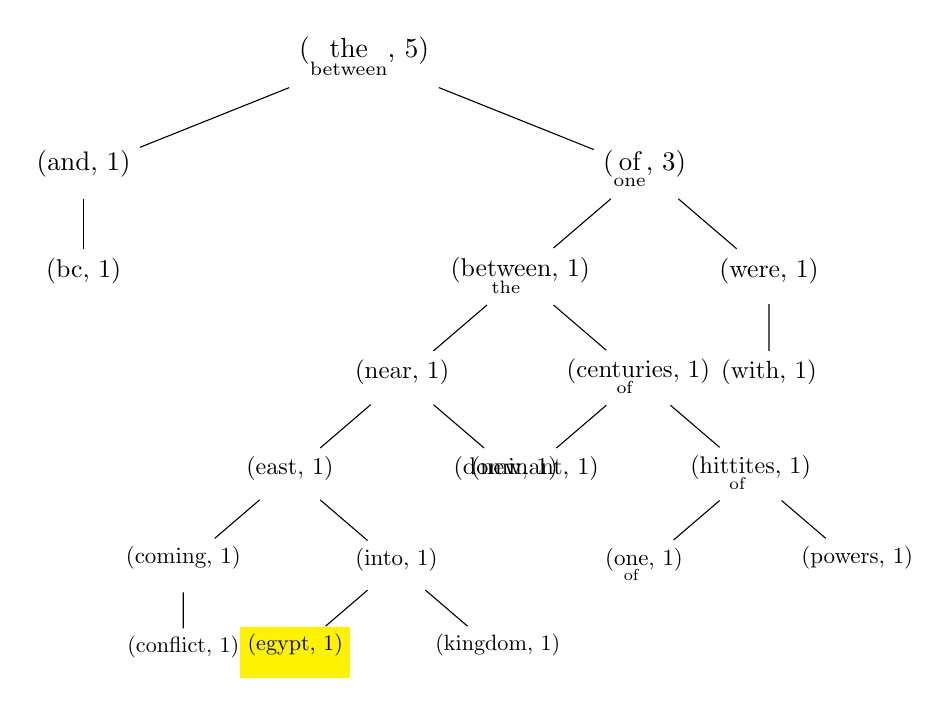
\begin{tikzpicture}
[
    level 1/.style={sibling distance=75mm, scale=1},
    level/.style={sibling distance=35mm, scale=.95},
]
\node [, scale=1.00]
{($\underset{\text{between}}{\text{the}}$, 5)} 
    child {node[, scale=0.97]
{($\underset{\text{}}{\text{and}}$, 1)} 
    child {node[, scale=0.93]
{($\underset{\text{}}{\text{bc}}$, 1)} 
}}    child {node[, scale=0.97]
{($\underset{\text{one}}{\text{of}}$, 3)} 
    child {node[, scale=0.93]
{($\underset{\text{the}}{\text{between}}$, 1)} 
    child {node[, scale=0.90]
{($\underset{\text{}}{\text{near}}$, 1)} 
    child {node[, scale=0.87]
{($\underset{\text{}}{\text{east}}$, 1)} 
    child {node[, scale=0.83]
{($\underset{\text{}}{\text{coming}}$, 1)} 
    child {node[, scale=0.80]
{($\underset{\text{}}{\text{conflict}}$, 1)} 
}}    child {node[, scale=0.83]
{($\underset{\text{}}{\text{into}}$, 1)} 
    child {node[fill=yellow, scale=0.80]
{($\underset{\text{}}{\text{egypt}}$, 1)} 
}    child {node[, scale=0.80]
{($\underset{\text{}}{\text{kingdom}}$, 1)} 
}}}    child {node[, scale=0.87]
{($\underset{\text{}}{\text{new}}$, 1)} 
}}    child {node[, scale=0.90]
{($\underset{\text{of}}{\text{centuries}}$, 1)} 
    child {node[, scale=0.87]
{($\underset{\text{}}{\text{dominant}}$, 1)} 
}    child {node[, scale=0.87]
{($\underset{\text{of}}{\text{hittites}}$, 1)} 
    child {node[, scale=0.83]
{($\underset{\text{of}}{\text{one}}$, 1)} 
}    child {node[, scale=0.83]
{($\underset{\text{}}{\text{powers}}$, 1)} 
}}}}    child {node[, scale=0.93]
{($\underset{\text{}}{\text{were}}$, 1)} 
    child {node[, scale=0.90]
{($\underset{\text{}}{\text{with}}$, 1)} 
}}};
\end{tikzpicture}
}
\end{center}

\end{tcolorbox}\section{« the »}
\begin{tcolorbox}[arc=5pt, colback=white!0, colframe=orange!50!black]
\infbox{
Insertion de \textbf{« the »}
}
\begin{center}
\tbox{
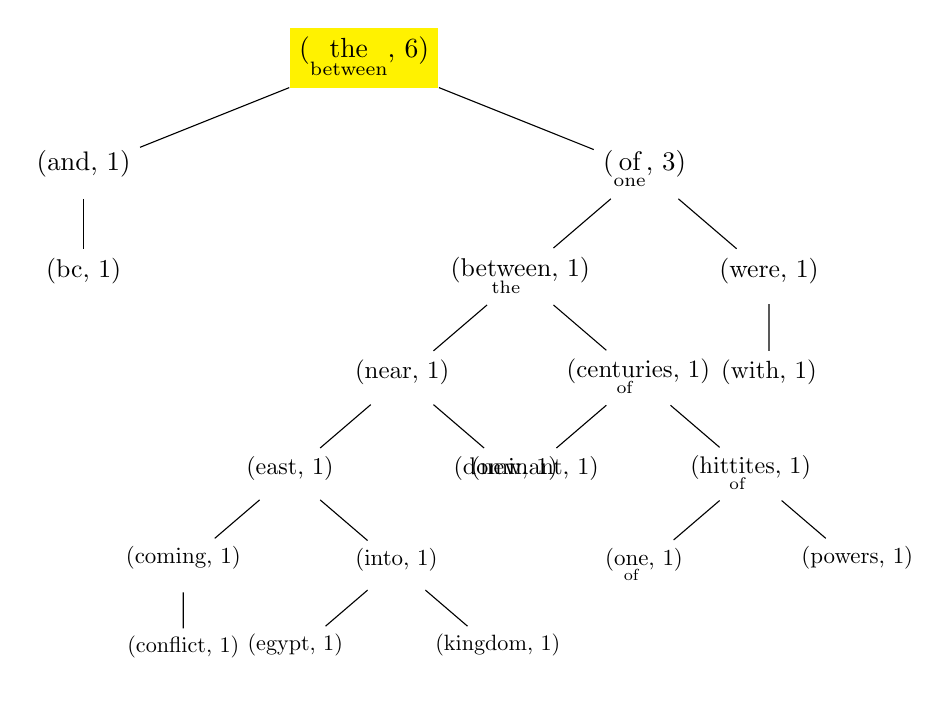
\begin{tikzpicture}
[
    level 1/.style={sibling distance=75mm, scale=1},
    level/.style={sibling distance=35mm, scale=.95},
]
\node [fill=yellow, scale=1.00]
{($\underset{\text{between}}{\text{the}}$, 6)} 
    child {node[, scale=0.97]
{($\underset{\text{}}{\text{and}}$, 1)} 
    child {node[, scale=0.93]
{($\underset{\text{}}{\text{bc}}$, 1)} 
}}    child {node[, scale=0.97]
{($\underset{\text{one}}{\text{of}}$, 3)} 
    child {node[, scale=0.93]
{($\underset{\text{the}}{\text{between}}$, 1)} 
    child {node[, scale=0.90]
{($\underset{\text{}}{\text{near}}$, 1)} 
    child {node[, scale=0.87]
{($\underset{\text{}}{\text{east}}$, 1)} 
    child {node[, scale=0.83]
{($\underset{\text{}}{\text{coming}}$, 1)} 
    child {node[, scale=0.80]
{($\underset{\text{}}{\text{conflict}}$, 1)} 
}}    child {node[, scale=0.83]
{($\underset{\text{}}{\text{into}}$, 1)} 
    child {node[, scale=0.80]
{($\underset{\text{}}{\text{egypt}}$, 1)} 
}    child {node[, scale=0.80]
{($\underset{\text{}}{\text{kingdom}}$, 1)} 
}}}    child {node[, scale=0.87]
{($\underset{\text{}}{\text{new}}$, 1)} 
}}    child {node[, scale=0.90]
{($\underset{\text{of}}{\text{centuries}}$, 1)} 
    child {node[, scale=0.87]
{($\underset{\text{}}{\text{dominant}}$, 1)} 
}    child {node[, scale=0.87]
{($\underset{\text{of}}{\text{hittites}}$, 1)} 
    child {node[, scale=0.83]
{($\underset{\text{of}}{\text{one}}$, 1)} 
}    child {node[, scale=0.83]
{($\underset{\text{}}{\text{powers}}$, 1)} 
}}}}    child {node[, scale=0.93]
{($\underset{\text{}}{\text{were}}$, 1)} 
    child {node[, scale=0.90]
{($\underset{\text{}}{\text{with}}$, 1)} 
}}};
\end{tikzpicture}
}
\end{center}

\end{tcolorbox}
\section{« middle »}
\begin{tcolorbox}[arc=5pt, colback=white!0, colframe=orange!50!black]
\infbox{
Insertion de \textbf{« middle »}
}
\begin{center}
\tbox{
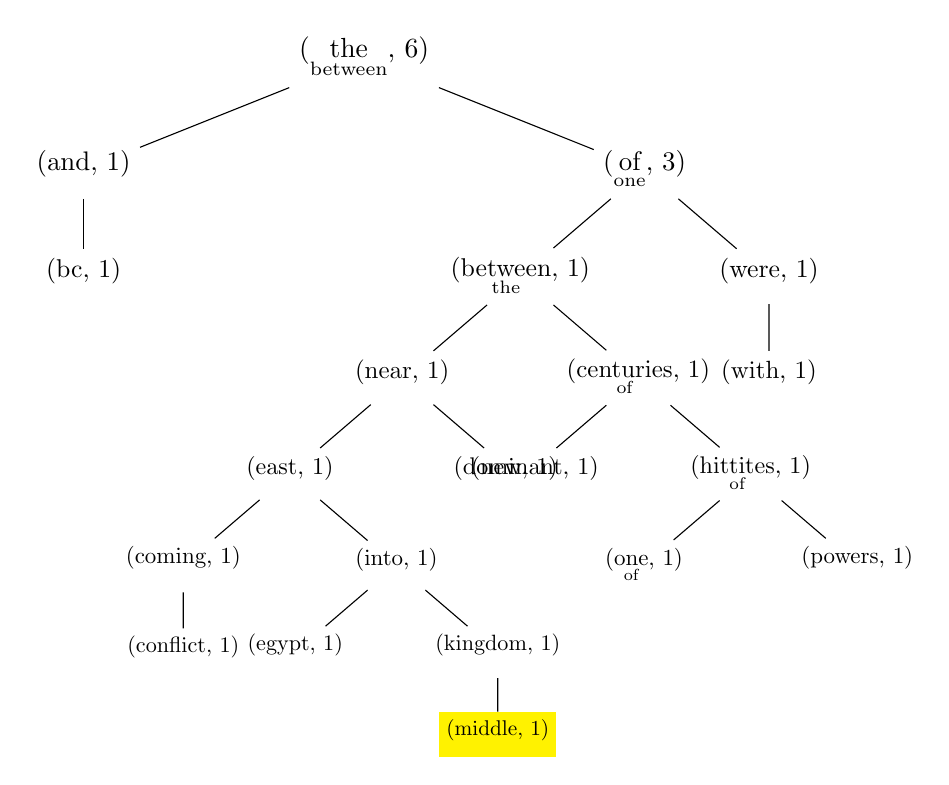
\begin{tikzpicture}
[
    level 1/.style={sibling distance=75mm, scale=1},
    level/.style={sibling distance=35mm, scale=.95},
]
\node [, scale=1.00]
{($\underset{\text{between}}{\text{the}}$, 6)} 
    child {node[, scale=0.97]
{($\underset{\text{}}{\text{and}}$, 1)} 
    child {node[, scale=0.93]
{($\underset{\text{}}{\text{bc}}$, 1)} 
}}    child {node[, scale=0.97]
{($\underset{\text{one}}{\text{of}}$, 3)} 
    child {node[, scale=0.93]
{($\underset{\text{the}}{\text{between}}$, 1)} 
    child {node[, scale=0.90]
{($\underset{\text{}}{\text{near}}$, 1)} 
    child {node[, scale=0.87]
{($\underset{\text{}}{\text{east}}$, 1)} 
    child {node[, scale=0.83]
{($\underset{\text{}}{\text{coming}}$, 1)} 
    child {node[, scale=0.80]
{($\underset{\text{}}{\text{conflict}}$, 1)} 
}}    child {node[, scale=0.83]
{($\underset{\text{}}{\text{into}}$, 1)} 
    child {node[, scale=0.80]
{($\underset{\text{}}{\text{egypt}}$, 1)} 
}    child {node[, scale=0.80]
{($\underset{\text{}}{\text{kingdom}}$, 1)} 
    child {node[fill=yellow, scale=0.77]
{($\underset{\text{}}{\text{middle}}$, 1)} 
}}}}    child {node[, scale=0.87]
{($\underset{\text{}}{\text{new}}$, 1)} 
}}    child {node[, scale=0.90]
{($\underset{\text{of}}{\text{centuries}}$, 1)} 
    child {node[, scale=0.87]
{($\underset{\text{}}{\text{dominant}}$, 1)} 
}    child {node[, scale=0.87]
{($\underset{\text{of}}{\text{hittites}}$, 1)} 
    child {node[, scale=0.83]
{($\underset{\text{of}}{\text{one}}$, 1)} 
}    child {node[, scale=0.83]
{($\underset{\text{}}{\text{powers}}$, 1)} 
}}}}    child {node[, scale=0.93]
{($\underset{\text{}}{\text{were}}$, 1)} 
    child {node[, scale=0.90]
{($\underset{\text{}}{\text{with}}$, 1)} 
}}};
\end{tikzpicture}
}
\end{center}

\end{tcolorbox}\section{« assyrian »}
\begin{tcolorbox}[arc=5pt, colback=white!0, colframe=orange!50!black]
\infbox{
Insertion de \textbf{« assyrian »}
}
\begin{center}
\tbox{
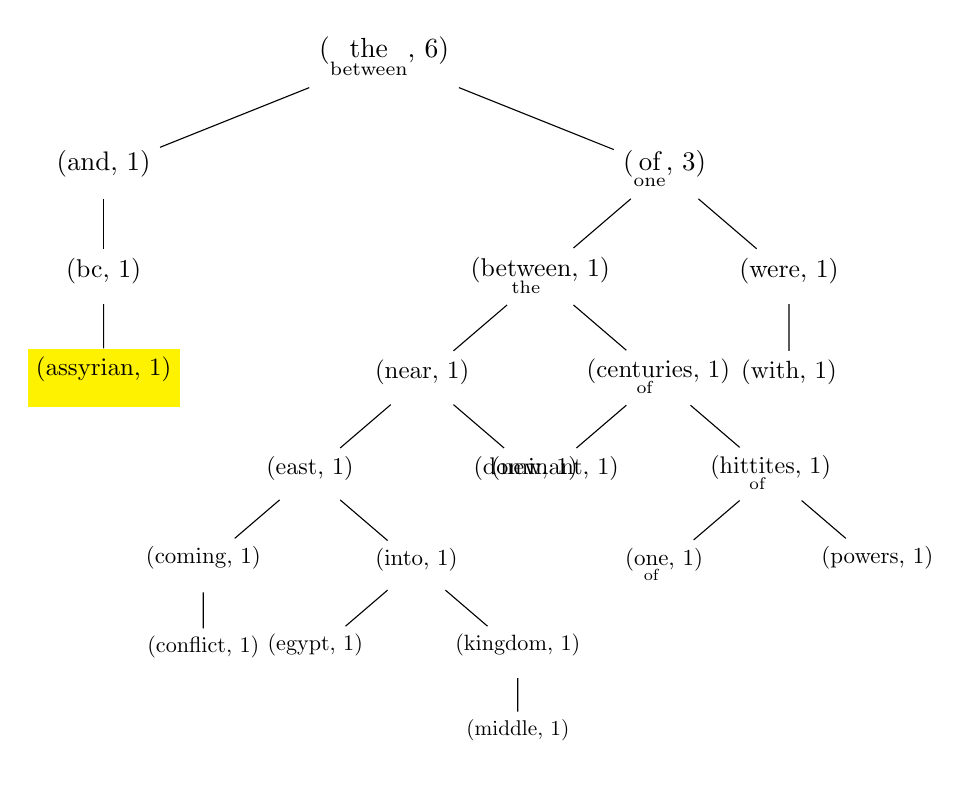
\begin{tikzpicture}
[
    level 1/.style={sibling distance=75mm, scale=1},
    level/.style={sibling distance=35mm, scale=.95},
]
\node [, scale=1.00]
{($\underset{\text{between}}{\text{the}}$, 6)} 
    child {node[, scale=0.97]
{($\underset{\text{}}{\text{and}}$, 1)} 
    child {node[, scale=0.93]
{($\underset{\text{}}{\text{bc}}$, 1)} 
    child {node[fill=yellow, scale=0.90]
{($\underset{\text{}}{\text{assyrian}}$, 1)} 
}}}    child {node[, scale=0.97]
{($\underset{\text{one}}{\text{of}}$, 3)} 
    child {node[, scale=0.93]
{($\underset{\text{the}}{\text{between}}$, 1)} 
    child {node[, scale=0.90]
{($\underset{\text{}}{\text{near}}$, 1)} 
    child {node[, scale=0.87]
{($\underset{\text{}}{\text{east}}$, 1)} 
    child {node[, scale=0.83]
{($\underset{\text{}}{\text{coming}}$, 1)} 
    child {node[, scale=0.80]
{($\underset{\text{}}{\text{conflict}}$, 1)} 
}}    child {node[, scale=0.83]
{($\underset{\text{}}{\text{into}}$, 1)} 
    child {node[, scale=0.80]
{($\underset{\text{}}{\text{egypt}}$, 1)} 
}    child {node[, scale=0.80]
{($\underset{\text{}}{\text{kingdom}}$, 1)} 
    child {node[, scale=0.77]
{($\underset{\text{}}{\text{middle}}$, 1)} 
}}}}    child {node[, scale=0.87]
{($\underset{\text{}}{\text{new}}$, 1)} 
}}    child {node[, scale=0.90]
{($\underset{\text{of}}{\text{centuries}}$, 1)} 
    child {node[, scale=0.87]
{($\underset{\text{}}{\text{dominant}}$, 1)} 
}    child {node[, scale=0.87]
{($\underset{\text{of}}{\text{hittites}}$, 1)} 
    child {node[, scale=0.83]
{($\underset{\text{of}}{\text{one}}$, 1)} 
}    child {node[, scale=0.83]
{($\underset{\text{}}{\text{powers}}$, 1)} 
}}}}    child {node[, scale=0.93]
{($\underset{\text{}}{\text{were}}$, 1)} 
    child {node[, scale=0.90]
{($\underset{\text{}}{\text{with}}$, 1)} 
}}};
\end{tikzpicture}
}
\end{center}

\end{tcolorbox}\section{« empire »}
\begin{tcolorbox}[arc=5pt, colback=white!0, colframe=orange!50!black]
\infbox{
Insertion de \textbf{« empire »}
}
\begin{center}
\tbox{
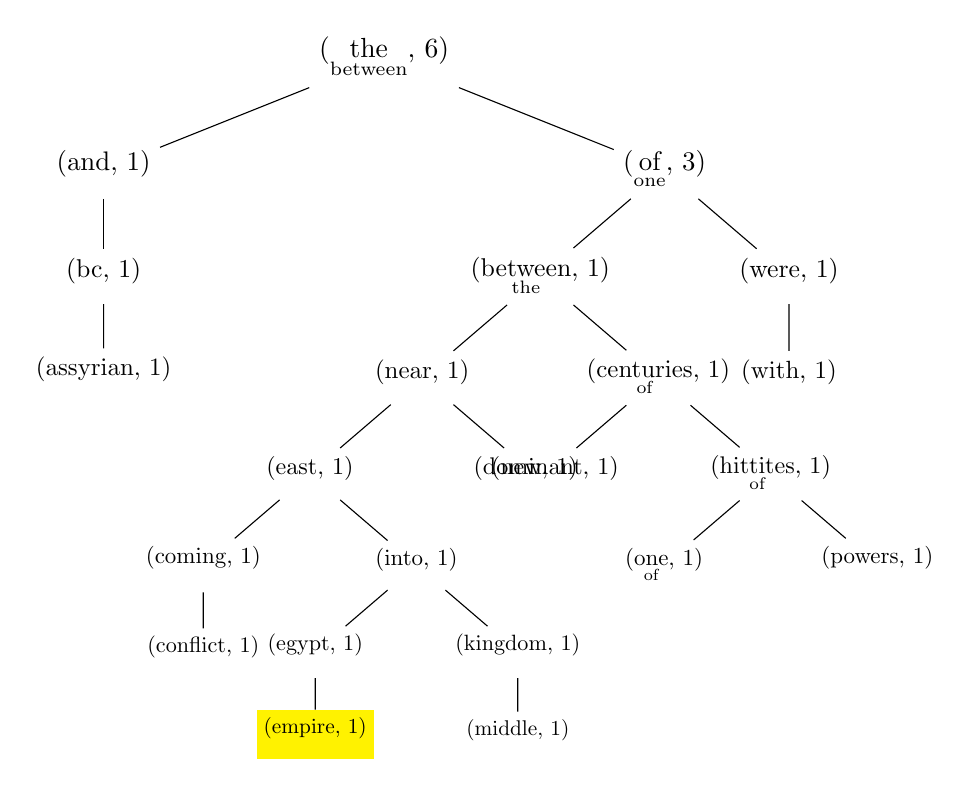
\begin{tikzpicture}
[
    level 1/.style={sibling distance=75mm, scale=1},
    level/.style={sibling distance=35mm, scale=.95},
]
\node [, scale=1.00]
{($\underset{\text{between}}{\text{the}}$, 6)} 
    child {node[, scale=0.97]
{($\underset{\text{}}{\text{and}}$, 1)} 
    child {node[, scale=0.93]
{($\underset{\text{}}{\text{bc}}$, 1)} 
    child {node[, scale=0.90]
{($\underset{\text{}}{\text{assyrian}}$, 1)} 
}}}    child {node[, scale=0.97]
{($\underset{\text{one}}{\text{of}}$, 3)} 
    child {node[, scale=0.93]
{($\underset{\text{the}}{\text{between}}$, 1)} 
    child {node[, scale=0.90]
{($\underset{\text{}}{\text{near}}$, 1)} 
    child {node[, scale=0.87]
{($\underset{\text{}}{\text{east}}$, 1)} 
    child {node[, scale=0.83]
{($\underset{\text{}}{\text{coming}}$, 1)} 
    child {node[, scale=0.80]
{($\underset{\text{}}{\text{conflict}}$, 1)} 
}}    child {node[, scale=0.83]
{($\underset{\text{}}{\text{into}}$, 1)} 
    child {node[, scale=0.80]
{($\underset{\text{}}{\text{egypt}}$, 1)} 
    child {node[fill=yellow, scale=0.77]
{($\underset{\text{}}{\text{empire}}$, 1)} 
}}    child {node[, scale=0.80]
{($\underset{\text{}}{\text{kingdom}}$, 1)} 
    child {node[, scale=0.77]
{($\underset{\text{}}{\text{middle}}$, 1)} 
}}}}    child {node[, scale=0.87]
{($\underset{\text{}}{\text{new}}$, 1)} 
}}    child {node[, scale=0.90]
{($\underset{\text{of}}{\text{centuries}}$, 1)} 
    child {node[, scale=0.87]
{($\underset{\text{}}{\text{dominant}}$, 1)} 
}    child {node[, scale=0.87]
{($\underset{\text{of}}{\text{hittites}}$, 1)} 
    child {node[, scale=0.83]
{($\underset{\text{of}}{\text{one}}$, 1)} 
}    child {node[, scale=0.83]
{($\underset{\text{}}{\text{powers}}$, 1)} 
}}}}    child {node[, scale=0.93]
{($\underset{\text{}}{\text{were}}$, 1)} 
    child {node[, scale=0.90]
{($\underset{\text{}}{\text{with}}$, 1)} 
}}};
\end{tikzpicture}
}
\end{center}

\end{tcolorbox}\section{« and »}
\begin{tcolorbox}[arc=5pt, colback=white!0, colframe=orange!50!black]
\infbox{
Insertion de \textbf{« and »}
}
\begin{center}
\tbox{
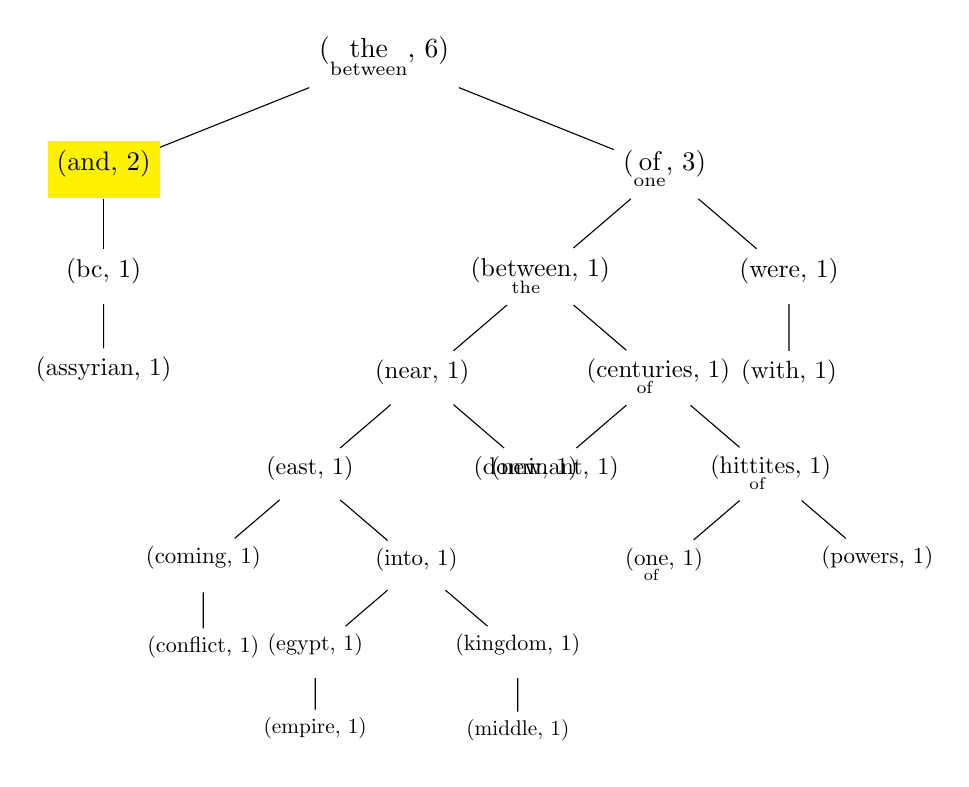
\begin{tikzpicture}
[
    level 1/.style={sibling distance=75mm, scale=1},
    level/.style={sibling distance=35mm, scale=.95},
]
\node [, scale=1.00]
{($\underset{\text{between}}{\text{the}}$, 6)} 
    child {node[fill=yellow, scale=0.97]
{($\underset{\text{}}{\text{and}}$, 2)} 
    child {node[, scale=0.93]
{($\underset{\text{}}{\text{bc}}$, 1)} 
    child {node[, scale=0.90]
{($\underset{\text{}}{\text{assyrian}}$, 1)} 
}}}    child {node[, scale=0.97]
{($\underset{\text{one}}{\text{of}}$, 3)} 
    child {node[, scale=0.93]
{($\underset{\text{the}}{\text{between}}$, 1)} 
    child {node[, scale=0.90]
{($\underset{\text{}}{\text{near}}$, 1)} 
    child {node[, scale=0.87]
{($\underset{\text{}}{\text{east}}$, 1)} 
    child {node[, scale=0.83]
{($\underset{\text{}}{\text{coming}}$, 1)} 
    child {node[, scale=0.80]
{($\underset{\text{}}{\text{conflict}}$, 1)} 
}}    child {node[, scale=0.83]
{($\underset{\text{}}{\text{into}}$, 1)} 
    child {node[, scale=0.80]
{($\underset{\text{}}{\text{egypt}}$, 1)} 
    child {node[, scale=0.77]
{($\underset{\text{}}{\text{empire}}$, 1)} 
}}    child {node[, scale=0.80]
{($\underset{\text{}}{\text{kingdom}}$, 1)} 
    child {node[, scale=0.77]
{($\underset{\text{}}{\text{middle}}$, 1)} 
}}}}    child {node[, scale=0.87]
{($\underset{\text{}}{\text{new}}$, 1)} 
}}    child {node[, scale=0.90]
{($\underset{\text{of}}{\text{centuries}}$, 1)} 
    child {node[, scale=0.87]
{($\underset{\text{}}{\text{dominant}}$, 1)} 
}    child {node[, scale=0.87]
{($\underset{\text{of}}{\text{hittites}}$, 1)} 
    child {node[, scale=0.83]
{($\underset{\text{of}}{\text{one}}$, 1)} 
}    child {node[, scale=0.83]
{($\underset{\text{}}{\text{powers}}$, 1)} 
}}}}    child {node[, scale=0.93]
{($\underset{\text{}}{\text{were}}$, 1)} 
    child {node[, scale=0.90]
{($\underset{\text{}}{\text{with}}$, 1)} 
}}};
\end{tikzpicture}
}
\end{center}

\end{tcolorbox}
\section{« the »}
\begin{tcolorbox}[arc=5pt, colback=white!0, colframe=orange!50!black]
\infbox{
Insertion de \textbf{« the »}
}
\begin{center}
\tbox{
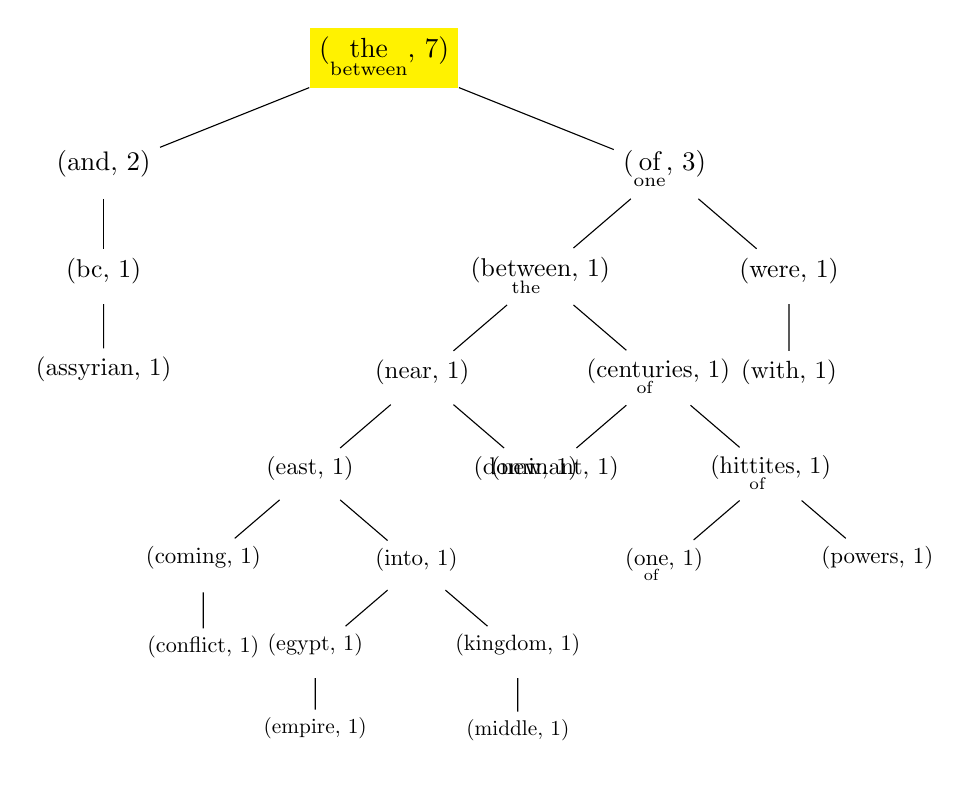
\begin{tikzpicture}
[
    level 1/.style={sibling distance=75mm, scale=1},
    level/.style={sibling distance=35mm, scale=.95},
]
\node [fill=yellow, scale=1.00]
{($\underset{\text{between}}{\text{the}}$, 7)} 
    child {node[, scale=0.97]
{($\underset{\text{}}{\text{and}}$, 2)} 
    child {node[, scale=0.93]
{($\underset{\text{}}{\text{bc}}$, 1)} 
    child {node[, scale=0.90]
{($\underset{\text{}}{\text{assyrian}}$, 1)} 
}}}    child {node[, scale=0.97]
{($\underset{\text{one}}{\text{of}}$, 3)} 
    child {node[, scale=0.93]
{($\underset{\text{the}}{\text{between}}$, 1)} 
    child {node[, scale=0.90]
{($\underset{\text{}}{\text{near}}$, 1)} 
    child {node[, scale=0.87]
{($\underset{\text{}}{\text{east}}$, 1)} 
    child {node[, scale=0.83]
{($\underset{\text{}}{\text{coming}}$, 1)} 
    child {node[, scale=0.80]
{($\underset{\text{}}{\text{conflict}}$, 1)} 
}}    child {node[, scale=0.83]
{($\underset{\text{}}{\text{into}}$, 1)} 
    child {node[, scale=0.80]
{($\underset{\text{}}{\text{egypt}}$, 1)} 
    child {node[, scale=0.77]
{($\underset{\text{}}{\text{empire}}$, 1)} 
}}    child {node[, scale=0.80]
{($\underset{\text{}}{\text{kingdom}}$, 1)} 
    child {node[, scale=0.77]
{($\underset{\text{}}{\text{middle}}$, 1)} 
}}}}    child {node[, scale=0.87]
{($\underset{\text{}}{\text{new}}$, 1)} 
}}    child {node[, scale=0.90]
{($\underset{\text{of}}{\text{centuries}}$, 1)} 
    child {node[, scale=0.87]
{($\underset{\text{}}{\text{dominant}}$, 1)} 
}    child {node[, scale=0.87]
{($\underset{\text{of}}{\text{hittites}}$, 1)} 
    child {node[, scale=0.83]
{($\underset{\text{of}}{\text{one}}$, 1)} 
}    child {node[, scale=0.83]
{($\underset{\text{}}{\text{powers}}$, 1)} 
}}}}    child {node[, scale=0.93]
{($\underset{\text{}}{\text{were}}$, 1)} 
    child {node[, scale=0.90]
{($\underset{\text{}}{\text{with}}$, 1)} 
}}};
\end{tikzpicture}
}
\end{center}

\end{tcolorbox}
\section{« empire »}
\begin{tcolorbox}[arc=5pt, colback=white!0, colframe=orange!50!black]
\infbox{
Insertion de \textbf{« empire »}
}
\begin{center}
\tbox{
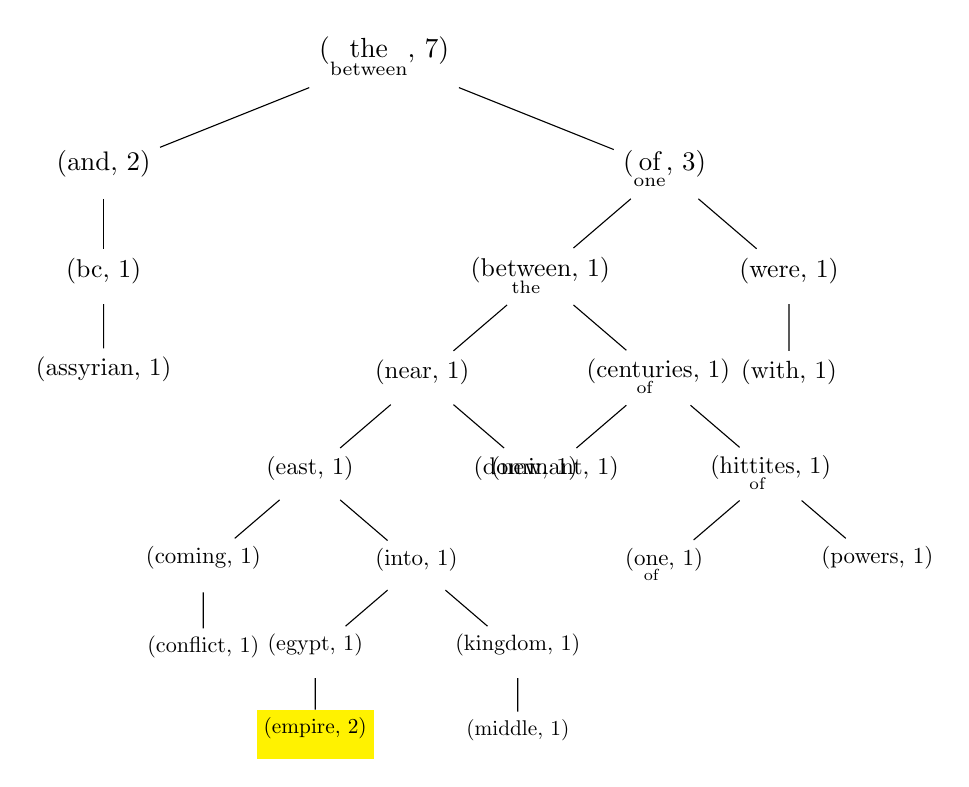
\begin{tikzpicture}
[
    level 1/.style={sibling distance=75mm, scale=1},
    level/.style={sibling distance=35mm, scale=.95},
]
\node [, scale=1.00]
{($\underset{\text{between}}{\text{the}}$, 7)} 
    child {node[, scale=0.97]
{($\underset{\text{}}{\text{and}}$, 2)} 
    child {node[, scale=0.93]
{($\underset{\text{}}{\text{bc}}$, 1)} 
    child {node[, scale=0.90]
{($\underset{\text{}}{\text{assyrian}}$, 1)} 
}}}    child {node[, scale=0.97]
{($\underset{\text{one}}{\text{of}}$, 3)} 
    child {node[, scale=0.93]
{($\underset{\text{the}}{\text{between}}$, 1)} 
    child {node[, scale=0.90]
{($\underset{\text{}}{\text{near}}$, 1)} 
    child {node[, scale=0.87]
{($\underset{\text{}}{\text{east}}$, 1)} 
    child {node[, scale=0.83]
{($\underset{\text{}}{\text{coming}}$, 1)} 
    child {node[, scale=0.80]
{($\underset{\text{}}{\text{conflict}}$, 1)} 
}}    child {node[, scale=0.83]
{($\underset{\text{}}{\text{into}}$, 1)} 
    child {node[, scale=0.80]
{($\underset{\text{}}{\text{egypt}}$, 1)} 
    child {node[fill=yellow, scale=0.77]
{($\underset{\text{}}{\text{empire}}$, 2)} 
}}    child {node[, scale=0.80]
{($\underset{\text{}}{\text{kingdom}}$, 1)} 
    child {node[, scale=0.77]
{($\underset{\text{}}{\text{middle}}$, 1)} 
}}}}    child {node[, scale=0.87]
{($\underset{\text{}}{\text{new}}$, 1)} 
}}    child {node[, scale=0.90]
{($\underset{\text{of}}{\text{centuries}}$, 1)} 
    child {node[, scale=0.87]
{($\underset{\text{}}{\text{dominant}}$, 1)} 
}    child {node[, scale=0.87]
{($\underset{\text{of}}{\text{hittites}}$, 1)} 
    child {node[, scale=0.83]
{($\underset{\text{of}}{\text{one}}$, 1)} 
}    child {node[, scale=0.83]
{($\underset{\text{}}{\text{powers}}$, 1)} 
}}}}    child {node[, scale=0.93]
{($\underset{\text{}}{\text{were}}$, 1)} 
    child {node[, scale=0.90]
{($\underset{\text{}}{\text{with}}$, 1)} 
}}};
\end{tikzpicture}
}
\end{center}

\end{tcolorbox}
\section{« of »}
\begin{tcolorbox}[arc=5pt, colback=white!0, colframe=orange!50!black]
\infbox{
Insertion de \textbf{« of »}
}
\begin{center}
\tbox{
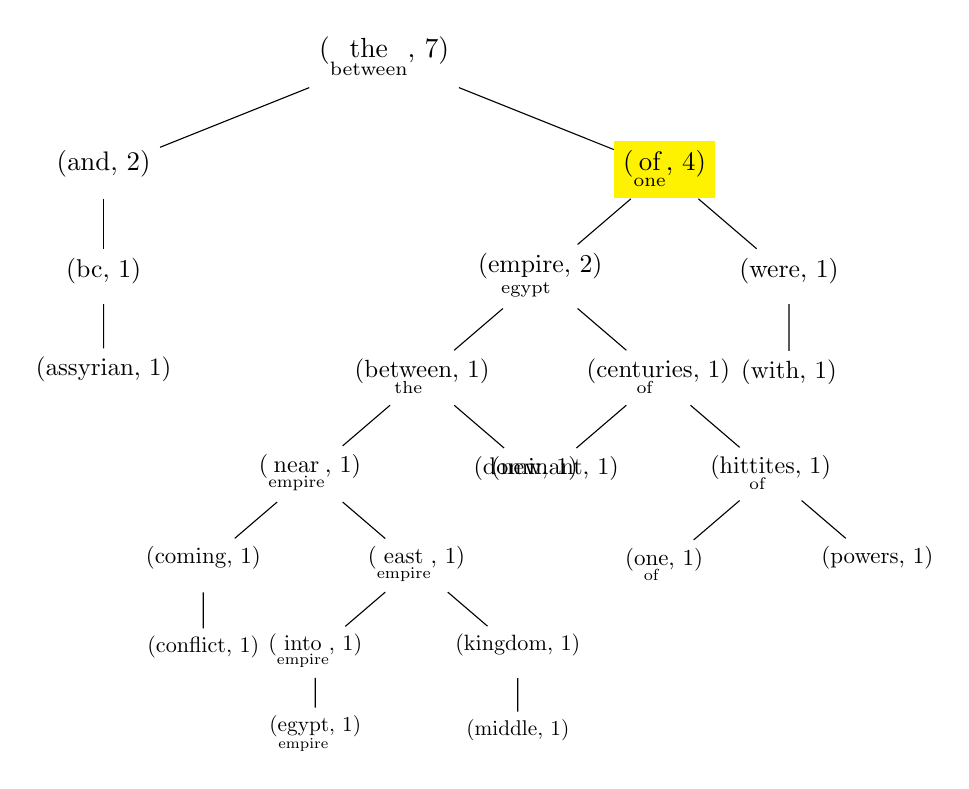
\begin{tikzpicture}
[
    level 1/.style={sibling distance=75mm, scale=1},
    level/.style={sibling distance=35mm, scale=.95},
]
\node [, scale=1.00]
{($\underset{\text{between}}{\text{the}}$, 7)} 
    child {node[, scale=0.97]
{($\underset{\text{}}{\text{and}}$, 2)} 
    child {node[, scale=0.93]
{($\underset{\text{}}{\text{bc}}$, 1)} 
    child {node[, scale=0.90]
{($\underset{\text{}}{\text{assyrian}}$, 1)} 
}}}    child {node[fill=yellow, scale=0.97]
{($\underset{\text{one}}{\text{of}}$, 4)} 
    child {node[, scale=0.93]
{($\underset{\text{egypt}}{\text{empire}}$, 2)} 
    child {node[, scale=0.90]
{($\underset{\text{the}}{\text{between}}$, 1)} 
    child {node[, scale=0.87]
{($\underset{\text{empire}}{\text{near}}$, 1)} 
    child {node[, scale=0.83]
{($\underset{\text{}}{\text{coming}}$, 1)} 
    child {node[, scale=0.80]
{($\underset{\text{}}{\text{conflict}}$, 1)} 
}}    child {node[, scale=0.83]
{($\underset{\text{empire}}{\text{east}}$, 1)} 
    child {node[, scale=0.80]
{($\underset{\text{empire}}{\text{into}}$, 1)} 
    child {node[, scale=0.77]
{($\underset{\text{empire}}{\text{egypt}}$, 1)} 
}}    child {node[, scale=0.80]
{($\underset{\text{}}{\text{kingdom}}$, 1)} 
    child {node[, scale=0.77]
{($\underset{\text{}}{\text{middle}}$, 1)} 
}}}}    child {node[, scale=0.87]
{($\underset{\text{}}{\text{new}}$, 1)} 
}}    child {node[, scale=0.90]
{($\underset{\text{of}}{\text{centuries}}$, 1)} 
    child {node[, scale=0.87]
{($\underset{\text{}}{\text{dominant}}$, 1)} 
}    child {node[, scale=0.87]
{($\underset{\text{of}}{\text{hittites}}$, 1)} 
    child {node[, scale=0.83]
{($\underset{\text{of}}{\text{one}}$, 1)} 
}    child {node[, scale=0.83]
{($\underset{\text{}}{\text{powers}}$, 1)} 
}}}}    child {node[, scale=0.93]
{($\underset{\text{}}{\text{were}}$, 1)} 
    child {node[, scale=0.90]
{($\underset{\text{}}{\text{with}}$, 1)} 
}}};
\end{tikzpicture}
}
\end{center}

\end{tcolorbox}

\end{document}